\documentclass[a4paper,10pt]{article}

\usepackage{color}
\usepackage{xcolor}
\usepackage{tikz}
\usepackage{amsmath}
\usepackage{amssymb}
\usepackage{amsthm}
\usepackage{graphicx}
\usepackage{mathtools}
\usepackage{wrapfig}
\usepackage{multirow}
\usepackage{comment}
\usepackage{natbib}
%\usepackage{float}
\usepackage{appendix}
\usepackage{subfig}
\usepackage{enumitem}
\usepackage{newfloat}
\usepackage[utf8]{inputenc}
\usepackage{floatrow}
\usepackage{bm}
\usepackage{geometry}

\geometry{a4paper,left=10mm,right=10mm,top=15mm,bottom=15mm}

\usetikzlibrary{calc}
\usetikzlibrary{fit}
\usetikzlibrary{decorations.shapes,shapes.misc,calc, positioning, hobby, backgrounds}

\tikzset{decorate sep/.style 2 args=
{decorate,decoration={shape backgrounds,shape=circle,shape size=#1,shape sep=#2}}}

%\DeclarePairedDelimiter{\floor}{\lfloor}{\rightfloor}
%\DeclarePairedDelimiter{\ceil}{\lceil}{\rceil}

\newcommand{\halflength}{\ensuremath{\floor{\frac{m}{2}}}}
\newcommand{\floor}[1]{\left \lfloor #1 \right \rfloor}
\newcommand{\ceil}[1]{\left \lceil #1 \right \rceil}

\newtheorem{theorem}{Theorem}[section]
\newtheorem{corollary}[theorem]{Corollary}
\newtheorem{lemma}[theorem]{Lemma}

\theoremstyle{definition}
\newtheorem{definition}[theorem]{Definition}

\theoremstyle{definition}
\newtheorem{example}[theorem]{Example}
 
\theoremstyle{remark}
\newtheorem*{remark}{Remark}

\theoremstyle{definition}
\newtheorem*{note}{Note}

\DeclareFloatingEnvironment[fileext=los,
    listname={List of Example Figures},
    name=Example Figure,
    placement=tbhp,
    within=section,]{examplefigure}

\DeclareFloatingEnvironment[fileext=los,
    listname={List of myFigures},
    name=Figure,
    placement=tbhp,
    within=section,]{myfigure}      

\title{A graph Patrol Problem with a random attacker and an observable patroller}
\date{\today}
\author{Thomas Lowbridge \\ School of Mathematical Sciences \\ University of Nottingham}

\bibliographystyle{plain}

\begin{document}

\pagestyle{empty}
{
  \renewcommand{\thispagestyle}[1]{}
  \maketitle
  \tableofcontents  
}
\clearpage
\pagestyle{plain}


\setlength{\parindent}{0pt}
\setlength{\parskip}{1em}

\newpage
\pagenumbering{arabic}
\section{Introduction to a random attacker patroller game with observation}
The model has a graph, $Q=(N,E)$, with a set of nodes labeled $1$ to $n$, $N=\{1,...,n \}$, and a set of edges linking these nodes. The adjacency matrix $a=(a_{i,j})_{i,j \in N}$, has $a_{i,j}=1$ if $i$ and $j$ are adjacent and $a_{i,j}=0$ if they are not adjacent. By definition we will use $a_{i,i}=1 \quad \forall i \in N$.


An attacker has some attack time for node $i$, called $X_{i}$ and chooses to attack node $i$ with some probability, $p_{i}$. The attackers arrive according to some Poisson process with rate $\Lambda$, so by Poisson thinning they arrive at node $i$ according to a Poisson process with rate $\lambda_{i}=\Lambda p_{i}$.

The patroller, uses some walk (with possible waiting) to patrol the graph.We assume that a patrollers walk is able to capture all attacks that have already begun, but not completed. But unlike the `normal' setting the past unit time, the attackers do not start their attacks and instead will wait for the patroller to leave. Each missed attack at node $i$ inccures a cost of $c_{i}$ to the patroller.

We can formulate the state space, as the delineation of separate nodes. $\Omega= \{ (\bm{s},\bm{v})= \quad | \quad s_{i}=1,2,... , v_{i}=0,1,2,... \quad \forall i \in N \}$. Where $\bm{s}=(s_{1},...,s_{n})$ has each $s_{i}$ represent the number of time periods since the last visit for that node $i$ and $\bm{v}=(v_{1},...,v_{n})$ has each $v_{i}$ represent the number of attackers present in the last time period when the node $i$ was last visited (i.e The number of attackers known to be beginning their attack $s_{i}$ time ago at node $i$).

\begin{myfigure}
\begin{center}
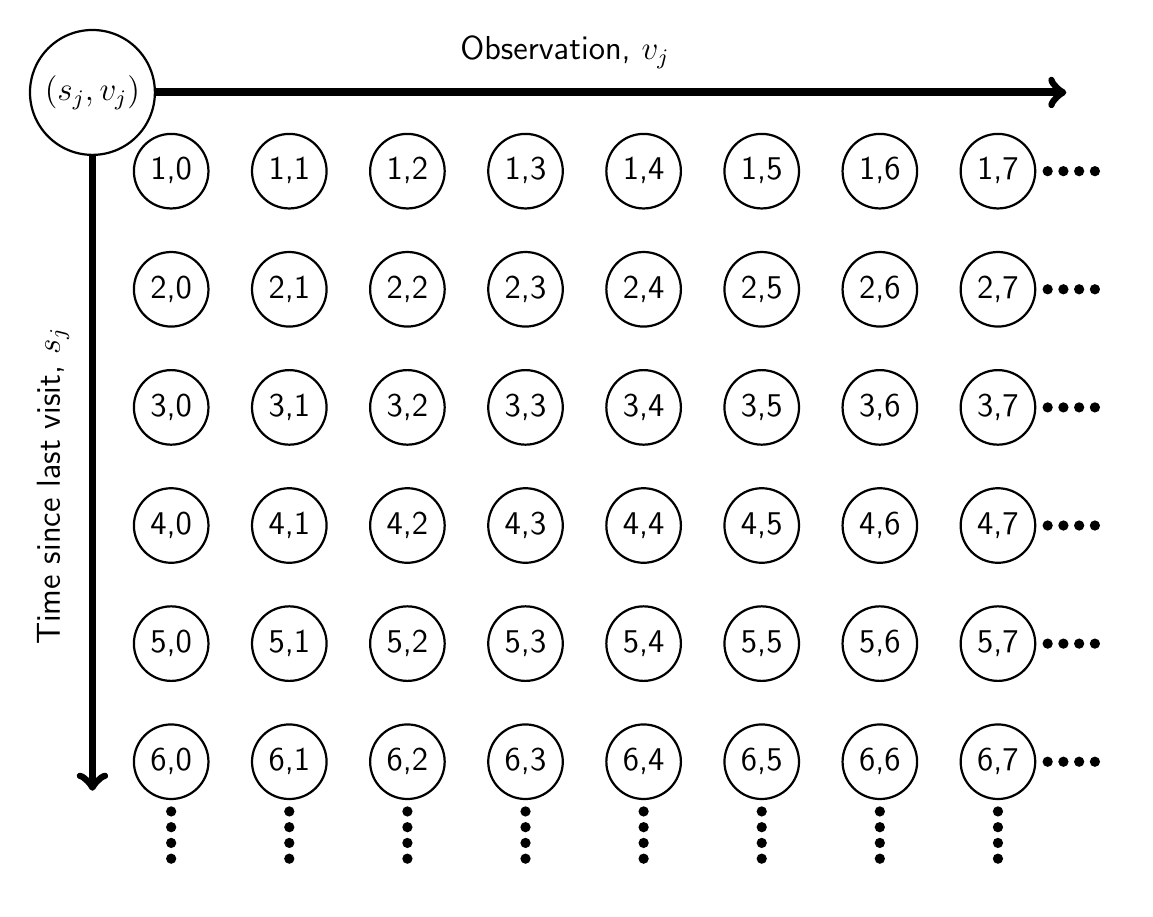
\begin{tikzpicture}[-,auto,node distance=1cm,
                    thick,main node/.style={circle,fill=white,draw,font=\sffamily\large,minimum size=0.5cm}]
 \foreach \x in {0,...,7}
    \foreach \y in {0,...,5} 
       {\pgfmathtruncatemacro{\label}{\x - 5 *  \y +21}
        \pgfmathtruncatemacro{\v}{\x}
        \pgfmathtruncatemacro{\s}{6-\y}
       \node [main node]  (\x\y) at (1.5*\x,1.5*\y) {\s,\v};} 

\node (XaxisLeft) [shift={(-0.5,1)}] at (05) {};
\node (XaxisRight) [shift={(1,1)}] at (75) {};

\node (YaxisBottom) [shift={(-1,-0.5)}] at (00) {};
\node (YaxisTop) [shift={(-1,1)}] at (05) {};

\draw[->,line width=1mm] (XaxisLeft)--(XaxisRight);
\draw[->,line width=1mm] (YaxisTop)--(YaxisBottom);

\node[font=\sffamily\large] (OLabel) [shift={(0.5,1.5)}] at (35) {Observation, $v_{j}$};
\node[font=\sffamily\large] (SLabel) [shift={(-1.5,0.5)}] at (02) {\rotatebox{90}{Time since last visit, $s_{j}$}};

\node[main node] (Example) [shift={(-1,1)}] at (05) {$(s_{j},v_{j})$};

\foreach \y in {0,...,5}
{\node (DottedStart\y) [shift={(0.5,0)}] at (7\y) {};
 \node (DottedEnd\y) [shift={(1.5,0)}] at (7\y) {};
 \draw[decorate sep={1mm}{2mm},fill] (DottedStart\y)--(DottedEnd\y);}
 
\foreach \x in {0,...,7}
{\node (\x DottedStart) [shift={(0,-0.5)}] at (\x0) {};
 \node (\x DottedEnd) [shift={(0,-1.5)}] at (\x0) {};
 \draw[decorate sep={1mm}{2mm},fill] (\x DottedStart)--(\x DottedEnd);
} 
\end{tikzpicture}
\end{center}
\caption{State space diagram}
\end{myfigure}

The $s_{i}$ increment by $1$ if the node is not visited upon each action, or if the node is visited reset to $s_{i}=1$. The $v_{i}$ do not change for nodes not visited, when a node is visited, the $v_{i}$ `reset' according to the Poisson distribution $Po(\lambda_{i} \times 1)=Po(\lambda)$. Due to $s_{i}=1$ if and only if the patroller is currently at this node, we will use $l(\bm{s})=\arg\min\limits_{i \in N} s_{i}$ to represent the current node.

As the future of the process is independent of its past, the process can be formulated as a Markov decision process(MDP), where at the end of the period, the patroller chooses which adjacent node to visit. Thus the action space is $\mathcal{A}=\{ j \, | \, a_{l(\bm{s}),j}=1 \}$, with a deterministic, stationary policy, $\pi: \Omega \rightarrow \mathcal{A}$.

The transitions of the MDP aren't entirely deterministic, $\bm{s}$ is purely deterministic, but $\bm{v}$ is partially probabilistic. In state $(\bm{s},\bm{v})$ with the decision to visit node $i \in \mathcal{A}$, then the state will transition to $(\widetilde{\bm{s}},\widetilde{\bm{v}})$ where $\widetilde{s}_{j}=s_{j}+1$ if $j \neq i$ and $\widetilde{s}_{j}=1$ if $j=i$ and $\widetilde{v}_{j}=v_{j}$ if $j \neq i$ and $v_{j} \sim Po(\lambda)$ if $j=i$.

To write down the cost function, which is dependent on the state $(\bm{s},\bm{v})$ and the action to visit node $i$ chosen, we will look at the expected cost of incurred at all nodes and sum these costs for the next time period.

\subsection{Derivation of the Cost function}
We will now work under the assumption that the patroller catches ongoing attacks at the end of the time period, but attacks arriving after their decision has been made to move to a node will be stopped and become the observed value.

We have two parts to the cost, the attacks which arrive and complete in the next time period and the cost of the locally-observed attacks that will finish.

First we will deal with the cost of attacks which arrive and complete. Then 
the cost for a node which is not being chosen to be visited we will get the `old' cost from the prior model i.e can arrive between $1$ and $s_{j}+1$ and finish in this next time period

This gives a value of
\begin{align*}
c_{j} \lambda_{j} \int_{0}^{s_{j}} P(t-1 < X_{j} \leq t) dt
=c_{j} \lambda_{j} \int_{s_{j}-1}^{s_{j}} P(X_{j} \leq t) dt
\end{align*}

However the cost for a node which is being chosen to be visited, will only have arrivals between $1$ and $s_{j}$ able to finish in this next time period (as the ones between $s_{j}$ and $s_{j}+1$ are `stopped' and become locally-observed attackers)

This gives a value of
\begin{align*}
c_{j} \lambda_{j} \int_{0}^{s_{j}-1} P(t < X_{j} \leq t+1) dt
&=c_{j} \lambda_{j} \int_{1}^{s_{j}} P(u-1 < X_{j} \leq u) du \\
&=c_{j} \lambda_{j} (\underbrace{\int_{0}^{s_{j}} P(u-1 < X_{j} \leq u) du}_{\text{Old amount}} - \underbrace{\int_{0}^{1} P(u-1 < X_{j} \leq u) du}_{\text{Losing the last period arriving and finishing}}) \\
&=c_{j} \lambda_{j} (\int_{s_{j}-1}^{s_{j}} P(X_{j} \leq u) du - \int_{0}^{1} P(X_{j} \leq u) du) \\
&=c_{j} \lambda_{j} (\int_{s_{j}-1}^{s_{j}} P(X_{j} \leq t) dt - \int_{0}^{1} P(X_{j} \leq t) dt)
\end{align*}

Now the contribution for the know local-observed attackers is just the expected number of them that finish in this time period that is their contribution is given by

\begin{align*}
c_{j} v_{j} P(s_{j}-1 < X_{j} \leq s_{j})
\end{align*}


Giving an overall cost contribution from node $j$ when the action to move to node $i$ is chosen in current state $(\bm{s},\bm{v})$.
\begin{align}
C_{j}(\bm{s},\bm{v},i)&= \begin{cases}
c_{j} (\lambda_{j} \int_{s_{j}-1}^{s_{j}} P(X_{j} \leq t) dt + v_{j} P(s_{j}-1 < X_{j} \leq s_{j})) \text{ for } i \neq j \\
c_{j} (\lambda_{j} (\int_{s_{j}-1}^{s_{j}} P(X_{j} \leq t) dt - \int_{0}^{1} P(X_{j} \leq t) dt)+v_{j} P(s_{j}-1 < X_{j} \leq s_{j}))  \text{ for } i=j \\
\end{cases} 
\end{align}

That is the only difference between having chosen the nodes is the effect on the cost is to remove the one time period closest to when we visit.
   
With $C(\bm{s},\bm{v},i)=\sum\limits_{j=1}^{n} C_{j}(\bm{s},\bm{v},i)$ being the cost function for the MDP.

\subsection{Bounding Problem}
We will now make the assumptions that $X_{j}$ is bounded and we will let
\begin{align*}
B_{j}=\min \{k \in \mathbb{N}_{0} \, | \, P(X_{j} \leq k)=1 \}
\end{align*}.
I.e $B_{j}$ is the least integer such that it is an upper bound for $X_{j}$. (we can think of this as the ceiling function on the real bound of  $X_{j}$ i.e if $X_{j} \leq RB_{j}$, where $RB_{j} \in \mathbb{R}$ then $B_{j}=\ceil{RB_{j}}$).
The cost function is the same for all $s_{j} \geq B_{j}+1$ so we will restrict our state space to $s_{j} \leq B_{j}+1$.

We will also limit the observation state space, from $Po(\lambda)$ for the observation transition and placing a bound on this Poisson distribution, named $b_{j}$, so we are now drawing from a truncated Poisson distribution, henceforth called $TPo(\lambda,b_{j})$. Then we can immediately say that the $v_{j} \leq b_{j}$ state is finite.

So our modified transition is $\widetilde{s_{j}}=\min(s_{j}+1,B_{j}+1)$ if $j \neq i$ and $\widetilde{s_{j}}=1$ if $i=j$. $\widetilde{v_{j}}=v_{j}$ if $i \neq j$ and $v_{j} \sim TPo(\lambda,b_{j})$ if $i=j$.

The truncated Poisson distribution, $TPo(\lambda,b)$ acts like normal Poisson for any value not equal to $b$, with the tails probability stored at $b$. That is $P(TPo(\lambda,b)=i)=\begin{cases}
P(Po(\lambda)=i) \text{ If } i \neq b \\
P(Po(\lambda) \geq b) \text{ If } i=b \\
0 \text{ Otherwise}
\end{cases}$

\begin{myfigure}
\begin{center}
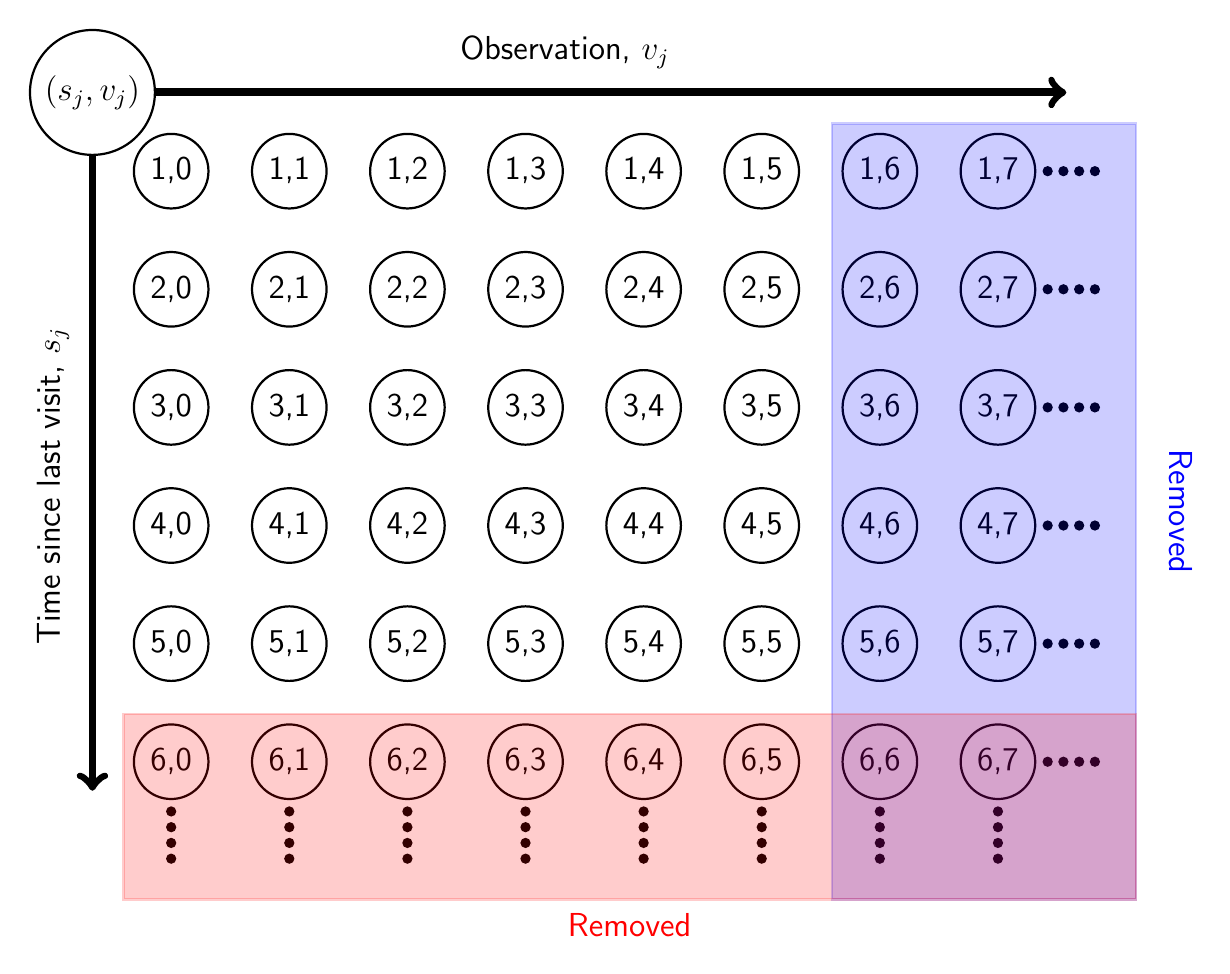
\begin{tikzpicture}[-,auto,node distance=1cm,
                    thick,main node/.style={circle,fill=white,draw,font=\sffamily\large,minimum size=0.5cm}]
 \foreach \x in {0,...,7}
    \foreach \y in {0,...,5} 
       {\pgfmathtruncatemacro{\label}{\x - 5 *  \y +21}
        \pgfmathtruncatemacro{\v}{\x}
        \pgfmathtruncatemacro{\s}{6-\y}
       \node [main node]  (\x\y) at (1.5*\x,1.5*\y) {\s,\v};} 

\node (XaxisLeft) [shift={(-0.5,1)}] at (05) {};
\node (XaxisRight) [shift={(1,1)}] at (75) {};

\node (YaxisBottom) [shift={(-1,-0.5)}] at (00) {};
\node (YaxisTop) [shift={(-1,1)}] at (05) {};

\draw[->,line width=1mm] (XaxisLeft)--(XaxisRight);
\draw[->,line width=1mm] (YaxisTop)--(YaxisBottom);

\node[font=\sffamily\large] (OLabel) [shift={(0.5,1.5)}] at (35) {Observation, $v_{j}$};
\node[font=\sffamily\large] (SLabel) [shift={(-1.5,0.5)}] at (02) {\rotatebox{90}{Time since last visit, $s_{j}$}};

\node[main node] (Example) [shift={(-1,1)}] at (05) {$(s_{j},v_{j})$};

\foreach \y in {0,...,5}
{\node (DottedStart\y) [shift={(0.5,0)}] at (7\y) {};
 \node (DottedEnd\y) [shift={(1.5,0)}] at (7\y) {};
 \draw[decorate sep={1mm}{2mm},fill] (DottedStart\y)--(DottedEnd\y);}
 
\foreach \x in {0,...,7}
{\node (\x DottedStart) [shift={(0,-0.5)}] at (\x0) {};
 \node (\x DottedEnd) [shift={(0,-1.5)}] at (\x0) {};
 \draw[decorate sep={1mm}{2mm},fill] (\x DottedStart)--(\x DottedEnd);
}

\node (Box1) [draw,thick,fit=(65) (60) (DottedEnd5) (DottedEnd0) (6DottedEnd) (7DottedEnd),fill,blue,opacity=0.2] {};

\node (Box2) [draw,thick,fit=(00) (70)(DottedEnd0) (0DottedEnd) (7DottedEnd),fill,red,opacity=0.2] {};

\node[font=\sffamily\large,color=blue] (Box1Text) [shift={(2.5,0)}] at (Box1) {\rotatebox{270}{Removed}};

\node[font=\sffamily\large,color=red] (Box2Text) [shift={(0,-1.5)}] at (Box2) {Removed};           

\end{tikzpicture}
\end{center}
\caption{State space diagram, with \textcolor{blue}{$b_{j}=5$} and \textcolor{red}{$B_{j}=4$} (e.g. $X_{j} \leq 3.7$)}
\end{myfigure}

Further reduction is possible as if $X_{j} \leq B_{j}$ then any observations $v_{j}$ which started $s_{j}-1$ time units ago (note that start at the end of a time period) is bound to have finished if $X_{j} \leq s_{j}-1$ and as $X_{j} \leq B_{j}$ it means $s_{j} \geq B_{j}+1$ implies all the waiting attacks have completed. So our `final' $s_{j}=B_{j}+1$ must have $v_{j}=0$.

\begin{example}
Say We have $X_{j} \sim U(0,3.7)$ then we have that $B_{j}=4$ and then as the cost function is the same for all $s_{j} \geq 4+1=5$ as we get
\begin{align*}
C_{j}(s_{j},v_{j},i)= c_{j} \lambda_{j}+0 \quad \forall j
\end{align*}

Also note at $s_{j}=5$ we have that $v_{j}=0$ as the attacks have had $4$ time periods respectively to complete and as at maximum it takes $3.7$ they must be complete.
\end{example}

So our new state space is further reduced to having only $(B_{j}+1,0)$ for node each node $j$.

So $\Omega= \{ (\bm{s},\bm{v}) | s_{i}=1,2,..,B_{i}+1 , v_{i}=0,1,...,b_{i} , \text{ if } s_{i} \in \{B_{i}+1 \} \text{ then } v_{i}=0 \, \forall i \in N \}$

\begin{myfigure}
\begin{center}
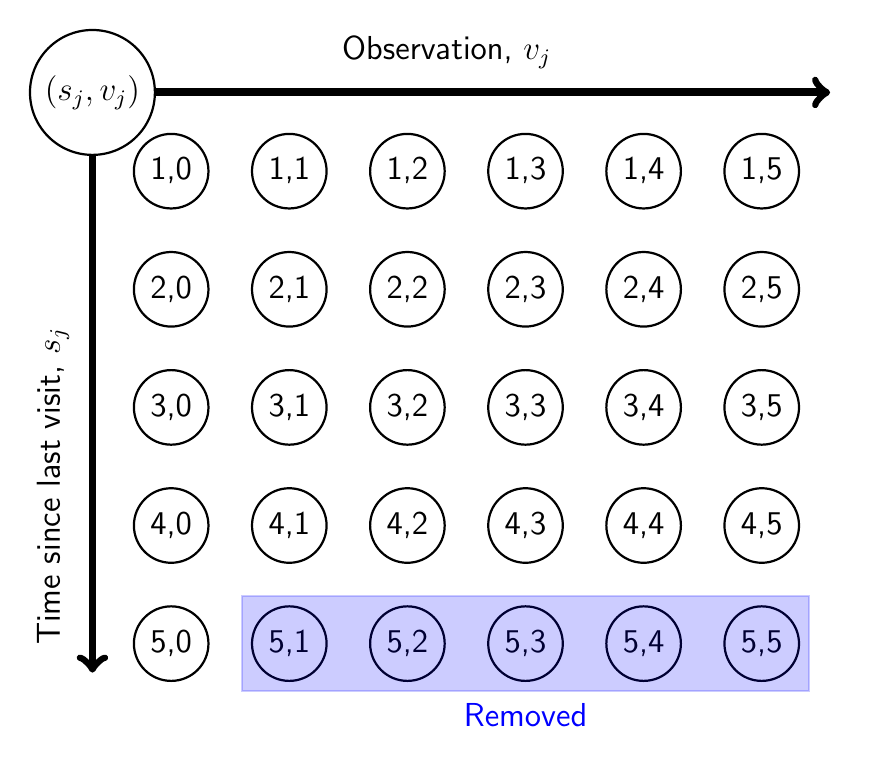
\begin{tikzpicture}[-,auto,node distance=1cm,
                    thick,main node/.style={circle,fill=white,draw,font=\sffamily\large,minimum size=0.5cm}]
 \foreach \x in {0,...,5}
    \foreach \y in {0,...,4} 
       {\pgfmathtruncatemacro{\label}{\x - 5 *  \y +21}
        \pgfmathtruncatemacro{\v}{\x}
        \pgfmathtruncatemacro{\s}{5-\y}
       \node [main node]  (\x\y) at (1.5*\x,1.5*\y) {\s,\v};} 

\node (XaxisLeft) [shift={(-0.5,1)}] at (04) {};
\node (XaxisRight) [shift={(1,1)}] at (54) {};

\node (YaxisBottom) [shift={(-1,-0.5)}] at (00) {};
\node (YaxisTop) [shift={(-1,1)}] at (04) {};

\draw[->,line width=1mm] (XaxisLeft)--(XaxisRight);
\draw[->,line width=1mm] (YaxisTop)--(YaxisBottom);

\node[font=\sffamily\large] (OLabel) [shift={(0.5,1.5)}] at (24) {Observation, $v_{j}$};
\node[font=\sffamily\large] (SLabel) [shift={(-1.5,0.5)}] at (01) {\rotatebox{90}{Time since last visit, $s_{j}$}};

\node[main node] (Example) [shift={(-1,1)}] at (04) {$(s_{j},v_{j})$};

\node (Box1) [draw,thick,fit=(10) (50),fill,blue,opacity=0.2] {};        

\node[font=\sffamily\large,color=blue] (Box1Text) [shift={(0,-0.9)}] at (Box1) {Removed};

\end{tikzpicture}
\end{center}
\caption{State space diagram, with $b_{j}=5$ and $B_{j}=4$ and further reduction of states with $s_{j}=5$ having to have $v_{j}=0$}
\end{myfigure}

With further modified transitions that if $\widetilde{s_{j}} =B_{j}+1$ then $\widetilde{v_{j}}=0$ for $i \neq j$ (Or equivalently if $s_{j}=B_{j}$ then $\widetilde{v_{j}}=0$ for $i \neq j$).

We will define $\phi_{s}(\bm{s},i)=\widetilde{\bm{s}}$, i.e the evolved $s$ states and similarly $\phi_{v}(\bm{s},\bm{v},i)=\widetilde{\bm{v}}$ i.e the evolved $v$ states.

\begin{note}
We note that the evolution of the $v$ states depends on the $s$ states, as if the $s_{j}=B_{j}$ then evolved state of $v_{j}$ becomes $0$. 
\end{note} 

\subsection{Problem formulation}
The objective of this MDP is to minimize the total long-run cost rate among the $n$ nodes of the graph. Our state space is finite because the attack time and local-observations are bounded above. The action space is finite because the number of nodes is finite. Hence we only consider deterministic , stationary policies (i.e we will always take the same action in the same state and time is irrelevant).

Unfortunately the state transitions are not fully deterministic, while the $s$ states evolve this way, the $v$ state which is visited will `reset' to a random number (drawn from our truncated poisson). We will define $\psi_{\pi}(\bm{s},\bm{v})=(\psi_{\pi,s}(\bm{s},\bm{v}),\psi_{\pi,v}(\bm{s},\bm{v}))=(\phi_{s}(\bm{s},\pi(\bm{s},\bm{v})),\bm{v}),\phi_{v}(\bm{s},\bm{v},\pi(\bm{s},\bm{v})))$.

That is $\psi_{\pi,s}(\bm{s},\bm{v})$ is purely deterministic, but $\psi_{\pi,v}(\bm{s},\bm{v})$ is partially random.

As the state space is finite and $\pi$ is a deterministic ,stationary policy, eventually we will visit the same state again. This should hold even though we are partially probabilistic. However the process will not regenerate itself, even though the same action will be taken we may end up in a different state state.

However for an initial state $(\bm{s}_{0},\bm{v}_{0})$ the policy $\pi$ does induce an indefinite,sequence of states $\{\psi_{\pi}^{k} (\bm{s}_{0},\bm{v}_{0}) \, | k=0,1,2... \}$ where $\psi_{\pi}^{k} (\bm{s}_{0},\bm{v}_{0})$ is the evolved state starting from the initial state after we apply $\pi$ $k$ times to the resulting state.

\begin{note}
We will have `cycles' of states which do repeat in the process, but we may jump to different cycles, due to the probabilistic nature of the evolved observations. This means cycles can be of different lengths.

That is to say we follow a selection of patrol patterns each for a different period of time. This selection depends on the probabilistic evolution. 

\end{note}

Therefore, if we apply the policy $\pi$ to an initial state $(\bm{s}_{0},\bm{v}_{0})$ we can write the long-run cost rate at node $i$ as

\begin{align*}
V_{i}(\pi,\bm{s}_{0},\bm{v}_{0})=\lim\limits_{N \rightarrow \infty} \frac{1}{N} \sum\limits_{k=0}^{N-1} C_{i}(\psi_{\pi}^{k}(\bm{s}_{0},\bm{v}_{0}),\pi(\psi_{\pi}^{k}(\bm{s}_{0},\bm{v}_{0})))
\end{align*}

We seek to determine the optimal long-run cost rate over all nodes, namely we seek the value

\begin{align}
C^{\text{OPT}}(\bm{s}_{0},\bm{v}_{0})= \min_{\pi \in \Pi} \sum\limits_{i=1}^{n} V_{i}(\pi,\bm{s}_{0},\bm{v}_{0})
\end{align}

Where $Pi$ is the class of deterministic, stationary patrol policies.

\begin{note}
A technical note is that we use the minimum rather than the infimum as $Pi$ is finite
\end{note}

If we take $C^{\text{OPT}}$ and divide it by the overall arrival rate, $\Lambda$ then we get the minimized long-run cost incurred for each attack. Furthermore if we set $c_{i}=1 \, \forall i \in N$ , then this ratio can be interpreted as the probability of not detecting an attack, i.e the evasion probability.

We will also note that while $V_{i}(\pi,\bm{s}_{0},\bm{v}_{0})$ depends on initial state $(\bm{s}_{0},\bm{v}_{0})$, the optimal cost rate $C^{\text{OPT}}(\bm{s}_{0},\bm{v}_{0})$ does not if the graph is connected. This is because from any initial state, we can construct a policy $\pi$ which produces our optimal selection of patrol patterns.

Hence we will drop the dependence on the initial state and the value of $C^{\text{OPT}}$ will be the same for every initial state. 

\section{Problem Relaxation}
We know look at relaxing our problem to easier to solve problems.

\subsection{Multiple Node problem}
We will now relax our class of problems to allow ourselves to visit multiple nodes in one time period, as long as the overall long-run visit rate is not greater than $1$. We will call this Problem the \textit{multiple node} (MN) problem. To extend ourselves to this problem we will create a new class of polices, $\Pi^{\text{MN}}$ which will allow the patroller to visit any set of nodes during the next timer period.

\begin{align*}
\pi : \Omega \rightarrow \{\bm{\alpha} \, | \, \alpha_{i} \in \{0,1 \} \text{ for } i=1,...,n \}
\end{align*}

Where $\alpha_{i}=1$ if the patroller will visit node $i$ in the next time period and $\alpha_{i}=0$ if the patroller will not visit node $i$ in the next time period. This patrol policy is more complex then those previously discussed and $\Pi \subset \Pi^{\text{MN}}$.

We now define the long-run rate at which the patroller visits node $i$, following $\pi$

\begin{align*}
\mu_{i}(\pi,\bm{s}_{0},\bm{v}_{0})=\lim\limits_{N \rightarrow \infty} \frac{1}{N} \sum\limits_{k=0}^{N-1} \alpha_{\psi_{\pi}^{k}(\bm{s}_{0},\bm{v}_{0}),i}
\end{align*}

We now impose the \textit{total-rate} constraint, that is the long-run overall visit rate to all nodes is no greater than 1. 

\begin{align*}
\sum\limits_{i=1}^{n} \mu_{i}(\pi,\bm{s}_{0},\bm{v}_{0}) \quad \forall (\bm{s}_{0},\bm{v}_{0}) \in \Omega
\end{align*}

and we denote the set of policies, which satisfy this constraint by

\begin{align*}
\Pi^{\text{TR}}=\left\{ \pi \in \Pi^{\text{MN}} \, \bigg| \, \sum\limits_{i=1}^{n} \mu_{i}(\pi,\bm{s}_{0},\bm{v}_{0}) \quad \forall (\bm{s}_{0},\bm{v}_{0}) \in \Omega \right\}
\end{align*}

Again $\Pi \subset \Pi^{\text{TR}}$

As discussed previously the optimal long-run cost rate does not depend on the initial state so we will drop the notation.

Therefore our relaxed problem can be formulated as

\begin{align*}
C^{\text{TR}}=\min_{\pi \in \Pi^{\text{TR}}} \sum\limits_{i=1}^{n} V_{i}(\pi)
\end{align*}

Hence due to this class of policies including the old class of policies, it is only possible to get a lower optimal value and hence $C^{\text{OPT}} \geq C^{\text{TR}}$.

\subsection{Lagrangian relaxation}
We now relax the problem again by incorporating the total rate constraint into the objective function, with a Lagrange multiplier, $\omega \geq 0$. This forms

\begin{align*}
C(\omega)&=\min_{\pi \in \Pi^{\text{MN}}} \left\{ \sum\limits_{i=1}^{n} V_{i}(\pi) + \omega \left( \sum\limits_{i=0}^{n} \mu_{i}(\pi) -1 \right) \right\} \\
&=\min_{\pi \in \Pi^{\text{MN}}} \sum\limits_{i=1}^{n} (V_{i}(\pi)+\omega \mu_{i}(\pi)) - \omega
\end{align*}

By incorporating the total-rate constraint as a Lagrange multiplier we can drop the constraint, so that the patroller can choose to visit any number of nodes in each time period (admittedly costing $\omega$).

We have that for any $\omega \geq 0$

\begin{align*}
C^{\text{TR}}=\min_{\pi \in \Pi^{\text{TR}}} \sum\limits_{i=1}^{n} V_{i}(\pi) &\geq \min_{\pi \in \Pi^{\text{TR}}} \left\{ \sum\limits_{i=1}^{n} V_{i}(\pi) + \omega \left( \sum\limits_{i=0}^{n} \mu_{i}(\pi) -1 \right) \right\} \\
&\geq \min_{\pi \in \Pi^{\text{MN}}} \left\{ \sum\limits_{i=1}^{n} V_{i}(\pi) + \omega \left( \sum\limits_{i=0}^{n} \mu_{i}(\pi) -1 \right) \right\}=C(\omega)
\end{align*}

The first inequality follows as the total-rate constraint is obeyed in $\Pi^{\text{TR}}$ and hence the $\omega \left( \sum\limits_{i=0}^{n} \mu_{i}(\pi) -1 \right) \leq 0$ and the second holds, as the total rate constraint is dropped and we have got a bigger state space, so we can only do better and hence possibly get a lower value.

Hence we have a string of inequalities $C^{\text{OPT}} \geq C^{\text{TR}} \geq C(\omega)$.

To solve the problem of finding $C(\omega)$ we can note that the problem can be split up into each node, for each node $i$ we want to minimize $V_{i}(\pi)+\omega \mu_{i}(\pi)$, where $\omega$ can be interpreted as the service charge when the patroller visits the node.

\subsection{Single node problem}
We will now focus on the problem of having a single node where we pay a service cost of $\omega$ to visit it. Namely we solve the objective function for $C(\omega)$ with the subscript for the node $i$ removed

\begin{align*}
\min_{\pi \in \Pi^{\text{MN}}} V(\pi) + \omega \mu(\pi)
\end{align*}

\section{Deterministic Attack time}
Consider the case where $X_{j}=x_{j}$, where $x_{j}$ is a constant (So $B_{j}=\ceil{x_{j}}$). So note that 
$$P(X_{j} \leq a)=\begin{cases}
1 \text{ if } a \geq x_{j} \\
0 \text{ if } a < x_{j}
\end{cases}$$

Then our cost function becomes

For $s_{j} < B_{j}$
\begin{align*}
C_{j}(\bm{s},\bm{v},i)=0
\end{align*}

For $s_{j}=B_{j}$
\begin{align*}
C_{j}(\bm{s},\bm{v},i)&=\begin{cases}
c_{j} \lambda_{j} \int_{B_{j}-1}^{B_{j}} P(X_{j} \leq t) dt + c_{j} v_{j} P(B_{j}-1 < X_{j} \leq B_{j}) \text{ for } i \neq j \\
c_{j} (\lambda_{j} (\int_{B_{j}-1}^{B_{j}} P(X_{j} \leq t) dt - \int_{0}^{1} P(X_{j} \leq t) dt) + c_{j} v_{j} P(B_{j}-1 < X_{j} \leq B_{j}) \text{ for } i=j \\
\end{cases} \\
&=\begin{cases}
c_{j} \lambda_{j} \int_{x_{j}}^{B_{j}} 1 dt + c_{j} v_{j} \times 1 \text{ for } i \neq j \\
c_{j} (\lambda_{j} (\int_{x_{j}}^{B_{j}} 1 dt - \int_{0}^{1} P(X_{j} \leq t) dt) + c_{j} v_{j} \times 1 \text{ for } i=j \\
\end{cases} 
\end{align*}

For $s_{j}=B_{j}+1$
\begin{align*}
C_{j}(\bm{s},\bm{v},i)&=\begin{cases}
c_{j} \lambda_{j} \int_{B_{j}}^{B_{j}+1} P(X_{j} \leq t) dt + c_{j} v_{j} P(B_{j} < X_{j} \leq B_{j}+1) \text{ for } i \neq j \\
c_{j} (\lambda_{j} (\int_{B_{j}}^{B_{j}+1} P(X_{j} \leq t) dt - \int_{0}^{1} P(X_{j} \leq t) dt) + c_{j} v_{j} P(B_{j}< X_{j} \leq B_{j}+1) \text{ for } i=j \\
\end{cases} \\
&=\begin{cases}
c_{j} \lambda_{j} \int_{B_{j}}^{B_{j}+1} 1 dt + c_{j} v_{j} \times 0 \text{ for } i \neq j \\
c_{j} (\lambda_{j} (\int_{B_{j}}^{B_{j}+1} 1 dt - \int_{0}^{1} P(X_{j} \leq t) dt) + c_{j} v_{j} \times 0 \text{ for } i=j \\
\end{cases} \\
\end{align*}

\begin{note}
The only such $s_{j}$ states are $s_{j}=\floor{B_{j}}+1,\floor{B_{j}}+2$
and in these cases we have that $v_{j}=0$ we infact have
\begin{align*}
C_{j}(\bm{s},\bm{v},i)=\begin{cases}
c_{j} \lambda_{j}(s_{j}-\floor{B_{j}}) \text { for } i \neq j \\
c_{j} \lambda_{j}(s_{j}-1-\floor{B_{j}}) \text{ for } i=j \\
\end{cases}
\end{align*}
\end{note}

Then we can further reduce the state space, as we choosing to visit later rather than earlier (as long as its not too late) allows us to possibly catch more (as we know when the attacks can start to finish). So we limit the state space with non-zero observed attackers to only have $s_{j}=\floor{B}+1$, as visiting at then gets any attacks caught when visiting at any $s_{j} < \floor{B}+1$.

So in the deterministic case $\Omega= \{(\floor{B}+1,v) \, | \, v=0,1,...,b \} \cup \{(\floor{B}+2,0) \}$.

\begin{myfigure}
\begin{center}
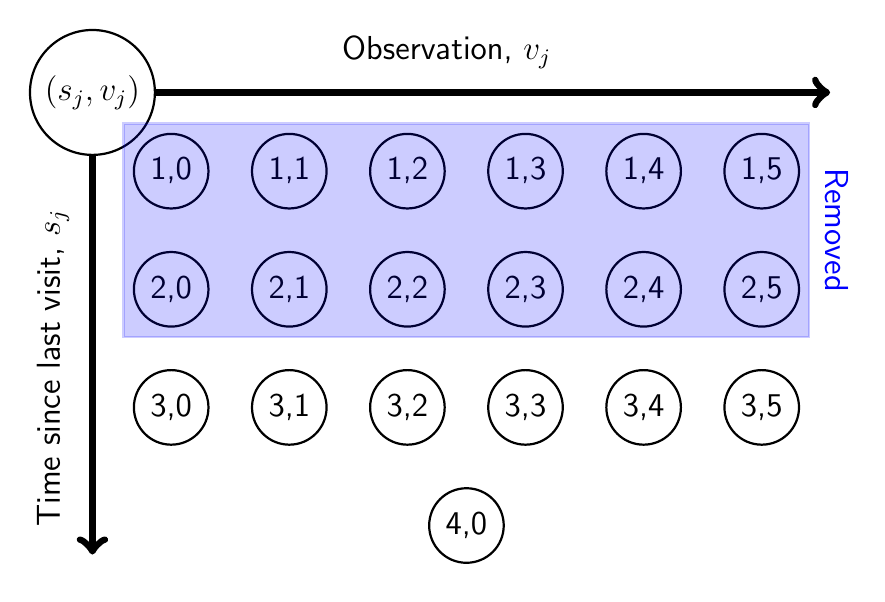
\begin{tikzpicture}[-,auto,node distance=1cm,
                    thick,main node/.style={circle,fill=white,draw,font=\sffamily\large,minimum size=0.5cm}]
 \foreach \x in {0,...,5}
    \foreach \y in {0,...,2} 
       {\pgfmathtruncatemacro{\label}{\x - 5 *  \y +21}
        \pgfmathtruncatemacro{\v}{\x}
        \pgfmathtruncatemacro{\s}{3-\y}
       \node [main node]  (\x\y) at (1.5*\x,1.5*\y) {\s,\v};}
       
\node[main node] (SpecialState) at (3.75,-1.5) {4,0};       

\node (XaxisLeft) [shift={(-0.5,1)}] at (02) {};
\node (XaxisRight) [shift={(1,1)}] at (52) {};

\node (YaxisBottom) [shift={(-1,-0.5)}] at (0,-1.5) {};
\node (YaxisTop) [shift={(-1,1)}] at (02) {};

\draw[->,line width=1mm] (XaxisLeft)--(XaxisRight);
\draw[->,line width=1mm] (YaxisTop)--(YaxisBottom);

\node[font=\sffamily\large] (OLabel) [shift={(0.5,1.5)}] at (22) {Observation, $v_{j}$};
\node[font=\sffamily\large] (SLabel) [shift={(-1.5,0.5)}] at (00) {\rotatebox{90}{Time since last visit, $s_{j}$}};

\node[main node] (Example) [shift={(-1,1)}] at (02) {$(s_{j},v_{j})$};

\node (Box1) [draw,thick,fit=(01) (51) (02) (52),fill,blue,opacity=0.2] {};        

\node[font=\sffamily\large,color=blue] (Box1Text) [shift={(4.7,0)}] at (Box1) {\rotatebox{270}{Removed}};
\end{tikzpicture}
\end{center}
\caption{Deterministic state space diagram, with $b_{j}=5$ and $B_{j}=4$}
\end{myfigure}

\begin{myfigure}
\begin{center}
\begin{tikzpicture}[-,auto,node distance=1cm,
                    thick,main node/.style={circle,fill=white,draw,font=\sffamily\large,minimum size=0.5cm}]
 \foreach \x in {0,...,5}
    \foreach \y in {0,...,0} 
       {\pgfmathtruncatemacro{\label}{\x - 5 *  \y +21}
        \pgfmathtruncatemacro{\v}{\x}
        \pgfmathtruncatemacro{\s}{3-\y}
       \node [main node]  (\x\y) at (1.5*\x,1.5*\y) {\s,\v};}
       
\node[main node] (SpecialState) at (3.75,-1.5) {4,0};       

\node (XaxisLeft) [shift={(-0.5,1)}] at (01) {};
\node (XaxisRight) [shift={(1,1)}] at (51) {};

\node (YaxisBottom) [shift={(-1,-0.5)}] at (0,-1.5) {};
\node (YaxisTop) [shift={(-1,1)}] at (01) {};

\draw[->,line width=1mm] (XaxisLeft)--(XaxisRight);
\draw[->,line width=1mm] (YaxisTop)--(YaxisBottom);

\node[font=\sffamily\large] (OLabel) [shift={(0.5,1.5)}] at (21) {Observation, $v_{j}$};
\node[font=\sffamily\large] (SLabel) [shift={(-2.4,0.5)}] at (00) {\rotatebox{90}{Time since last visit, $s_{j}$}};

\node[main node] (Example) [shift={(-1,1)}] at (01) {$(s_{j},v_{j})$};

\end{tikzpicture}
\end{center}
\caption{Final deterministic, with $b_{j}=5$ and $B_{j}=4$}
\end{myfigure}

We will first have a concrete argument as to why the decision is always to wait when in a state $(s,v)$ with $s < \floor{B}+1$. From this position consider the policy $\pi_{k}$ which waits $k$ time periods and then renews and follows the optimal policy, $\sigma$, with $k=0,...,\floor{B}+1-s$.

Using such a policy will get us that
\begin{equation}
V_{n}^{\pi_{k}}(x,v)=\omega + E[V_{n-k-1}^{\sigma}(\theta)]
\end{equation}

where $\theta$ is the state upon renewal (i.e it is the state $(1,V) \sim (1,TPo(\lambda))$.

Now we will pick policy $\pi_{k+1}$ over $\pi_{k}$ (or be indifferent) if

\begin{align*}
&\lim\limits_{n \rightarrow \infty} V_{n}^{\pi_{k}} (x,v) - V_{n}^{\pi_{k+1}}(x,v) \geq 0 \\
& \iff \lim\limits_{n \rightarrow \infty} E[V_{n-k}^{\sigma}(\theta) - V_{n-k-1}^{\sigma} (\theta)] \geq 0 \\
& \iff g \geq 0
\end{align*}

Where $g$ is the average long-run costs of the system, coming from $V_{n}(x,v)=ng + \phi(x,v)$ for large $n$, and $\phi(x,v)$ is some initial bias for not starting in equilibrium from the initial state $(x,v)$.

Now as the Dynamic Programming only has positive costs, it is impossible for $g < 0$. So we have that $g \geq 0$, so it is better to pick policy $\pi_{k+1}$ over $\pi_{k}$, as this argument holds for all $k=0,...,\floor{B}+1-s$ (and all $v$) it is best to wait till $(\floor{B}+1,v)$ before making a decision.

This formally shows the removal of the prior states.

Now we will skip to the state $(\floor{B}+2,0)$ and suggest again a policy $\pi_{k}$ which waits $k$ time periods before renewing and then follows some optimal policy, $\sigma$.

Using such a policy will get us
\begin{equation}
V_{n}^{\pi_{k}}(x,v)= \omega +c \lambda k + E[V_{n-k-1}^{\sigma}(\theta)]
\end{equation}

And again we will pick a policy $\pi_{k+1}$ over $\pi_{k}$ (or be indifferent) if

\begin{align*}
&\lim\limits_{n \rightarrow \infty} V_{n}^{\pi_{k}} (\floor{B}+2,0) - V_{n}^{\pi_{k+1}}(\floor{B}+2,0) \geq 0 \\
& \iff \lim\limits_{n \rightarrow \infty} -c \lambda + E[V_{n-k}^{\sigma}(\theta) - V_{n-k-1}^{\sigma}(\theta)] \geq 0 \\
& \iff g \geq c \lambda
\end{align*}

So hence if $g \geq c \lambda$ we will wait forever, as this has no dependence on $k$.

We will now argue that $g_{max}=c \lambda$, that is at worst the  long-run average cost is $c \lambda$. This can be seen by the strategy $\pi_{neg}$, a strategy which never renews no matter what state we are in. I.e the patroller neglects the node. We will have that, for large n

\begin{align*}
V_{n}^{\pi_{neg}}(x,v)=n c \lambda + \phi(x,v)
\end{align*}

We can observe this by looking at the actual decay of the process, under a policy that never renews

\begin{align*}
V_{n}^{\pi_{neg}}(x,v)=& V_{n-(\floor{B}+2-x)}^{\pi_{neg}} + \phi(x,v)
&=(n-(\floor{B}+2-x)) c \lambda + phi(x,v)
\end{align*}

Where $\phi(x,v)= \underbrace{v c \lambda}_{\text{Observed finishing}} + \underbrace{(1-R) c \lambda}_{\text{arrivals that finish}}$ ($R=B-\floor{B}$) is the `transfer'/bias of moving from the initial state to $(\floor{B}=2,1)$.

Hence for any service cost, $\omega$ we can achieve a $g= c \lambda$. So we will always be in the case of $g \leq c \lambda$ and hence we will renew if we hit the state $(\floor{B}+2,0)$ and hence for a state $(\floor{B}+1,v)$ we have two types of policy, $\pi_{0}$ a policy which renews now and then follows some optimal policy $\sigma$ or policy, $\pi_{1}$ which waits one period until $(\floor{B}+2,0)$ and then renews and follows some optimal policy $\sigma$.

So we will choice to renew now over waiting if

\begin{align*}
&\lim\limits_{n \rightarrow \infty} V_{n}^{\pi_{1}} (\floor{B}+1,v) - V_{n}^{\pi_{0}}(\floor{B}+1,v) \geq 0 \\
& \iff \lim\limits_{n \rightarrow \infty} (\floor{B}-B+1) c \lambda + v c + E[V_{n-1}^{\sigma}(\floor{B+2},0)] - (\omega + E[V_{n-1}^{\sigma}(\theta)]) \geq 0 \\
& \iff \lim\limits_{n \rightarrow \infty} (\floor{B}-B+1) c \lambda + v c  + E[ \omega + V_{n-2}^{\sigma}(\theta)] - \omega - E[V_{n-1}^{\sigma}(\theta)] \geq 0 \\
& \iff \lim\limits_{n \rightarrow \infty} (\lambda(\floor{B}-B+1)+v) c + E[V_{n-2}^{\sigma}(\theta) - V_{n-1}^{\sigma}(\theta)] \geq 0 \\
& \iff (1-R+v)c \lambda - g \geq 0 \\
& \iff g \leq c (\lambda(1-R)+v) 
\end{align*}

So we renew now if $g \leq (\lambda(1-R)+v)c$, as we are guaranteed that $g \leq c \lambda$ we are clearly in this region unless $\lambda R-v \geq 0 \iff v \leq \lambda R $, so if we will renew in $v$ we definitely renew in $v+1,v+2,...,b$. Their is some critical value, $v_{\text{crit}}=\ceil{\frac{g}{c}+ \lambda (R-1)}$ such that for $v \geq v_{\text{crit}}$ we renew immediately and for $v < v_{\text{crit}}$ we wait one time period and renew.

We have two special cases for $g$, that is when we always renew immediately or always wait then renew, these are $g \leq  c \lambda(1-R)$ (i.e we renew for all $v$ if we renew for $v=0$) and $g \geq c (\lambda(1-R)+b)$ (i.e we always wait then renew for all $v$ if we wait for $v=b$)

However between these regions, we have a divide of the nodes into a set we renew immediately and a set we wait then renew.

\begin{myfigure}
\begin{center}
\begin{tikzpicture}[-,auto,node distance=1cm,
                    thick,main node/.style={circle,fill=white,draw,font=\sffamily\large,minimum size=0.5cm}]
 \foreach \x in {0,...,5}
    \foreach \y in {0,...,0} 
       {\pgfmathtruncatemacro{\label}{\x - 5 *  \y +21}
        \pgfmathtruncatemacro{\v}{\x}
        \pgfmathtruncatemacro{\s}{3-\y}
       \node [main node]  (\x\y) at (1.5*\x,1.5*\y) {\s,\v};}
       
\node[main node] (SpecialState) at (3.75,-1.5) {4,0};       

\node (XaxisLeft) [shift={(-0.5,1)}] at (01) {};
\node (XaxisRight) [shift={(1,1)}] at (51) {};

\node (YaxisBottom) [shift={(-1,-0.5)}] at (0,-1.5) {};
\node (YaxisTop) [shift={(-1,1)}] at (01) {};

\draw[->,line width=1mm] (XaxisLeft)--(XaxisRight);
\draw[->,line width=1mm] (YaxisTop)--(YaxisBottom);

\node[font=\sffamily\large] (OLabel) [shift={(0.5,1.5)}] at (21) {Observation, $v$};
\node[font=\sffamily\large] (SLabel) [shift={(-2.4,0.5)}] at (00) {\rotatebox{90}{Time since last visit, $s$}};

\node[main node] (Example) [shift={(-1,1)}] at (01) {$(s,v)$};

\node (Topbarrier) [shift={(0.8,1)}] at (10) {};
\node (Bottombarrier) [shift={(0.8,-1)}] at (10) {};

\draw (Topbarrier)--(Bottombarrier);

\node (Barrierlabel) [shift={(0,0.2)}] at (Topbarrier) {$g=2.8$};

\node (Box1) [draw,thick,fit=(00) (10),fill,blue,opacity=0.2] {};

\node[blue] (Box1Label) [shift={(0,-1)}] at (Box1) {Wait then renew};

\node (Box2) [draw,thick,fit=(20) (50),fill,red,opacity=0.2] {};

\node[red] (Box2Label) [shift={(0,-1)}] at (Box2) {Renew now};

\end{tikzpicture}
\end{center}
\caption{With $c=\lambda=1$, $B=4.4 \implies R=0.4$ so $v_{\text{crit}}=2$ when $2.6 \leq g < 3.6$ (e.g $g=2.8$)}
\label{Figure: example of region splitting}
\end{myfigure}

However we are assuming we are in the case of $g \leq c \lambda$ for so the example \ref{Figure: example of region splitting} we cannot have a situation as $g_{\text{max}}=1$. Really in this case we would just follow the neglecting strategy, $\pi_{\text{neg}}$.

We really need to split the region for $g$ (which is bounded above by $c \lambda$) into different $v=v_{\text{crit}}$.

Say now we have that $b > \lambda R $ then we have some $v_{max}=\max \{ v \in \{ 0,1,...,b+1 \} \, | \, v \leq \lambda R \}$ , some critical maximum (as at some point we will turn on the neglecting strategy)

\begin{note}
$v_{\text{max}}=0$ means we always renew and $v_{\text{max}}=b+1$ means we never renew.
\end{note}

We do by having
\begin{itemize}
\item $v_{\text{crit}}=0$ if $g \leq c \lambda (1-R)$
\item $v_{\text{crit}}=k$ if $c \lambda (1-R) +c(k-1) < g \leq c \lambda (1-R)+ kc$ for $k=1,....,v_{\text{max}}-1$
\item $v_{\text{crit}}=v_{\text{max}}$ if $c \lambda (1-R) + c(v_{\text{max}}-1) < g \leq c \lambda$
\end{itemize}

Let us say that our $v_{\text{crit}}=k$ then we have that

\begin{align*}
g_{k}(\omega)&=\frac{\text{Expected cost per renewal}}{\text{Expected renewal length}} \\
&= \frac{\omega P(TPo(\lambda,b) \geq k) + (\omega + c \lambda (1-R )) P(TPo(\lambda,b)=0)+...+(\omega + c \lambda (1-R)) P(TPo(\lambda,b)=k-1)}{(\floor{B}+1)P(TPo(\lambda,b) \geq k) + (\floor{B}+2)P(TPo(\lambda,b) \leq k-1)} \\
&=\frac{\omega P(TPo(\lambda,b) \geq k) + (\omega + c \lambda (1-R))P(TPo(\lambda) \leq k-1) + c \sum\limits_{i=0}^{k-1} i P(TPo(\lambda,b)=i)}{(\floor{B}+1)P(TPo(\lambda,b) \geq k) + (\floor{B}+2)(1-P(TPo(\lambda,b) \geq k))} \\
&= \frac{\omega - c \lambda (1-R) P(TPo(\lambda,b) \geq k) +  \sum\limits_{i=0}^{k-1} i P(TPo(\lambda,b)=i)}{\floor{B}+2-P(TPo(\lambda,b) \geq k)}
\end{align*}

\begin{myfigure}
\begin{center}
\resizebox{.6\textwidth}{!}{
% Created by tikzDevice version 0.10.1 on 2018-02-26 10:34:12
% !TEX encoding = UTF-8 Unicode
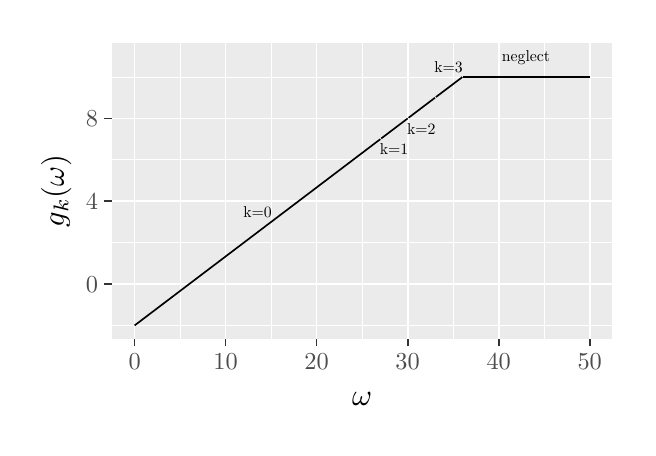
\begin{tikzpicture}[x=1pt,y=1pt]
\definecolor{fillColor}{RGB}{255,255,255}
\path[use as bounding box,fill=fillColor,fill opacity=0.00] (0,0) rectangle (216.81,144.54);
\begin{scope}
\path[clip] (  0.00,  0.00) rectangle (216.81,144.54);
\definecolor{drawColor}{RGB}{255,255,255}
\definecolor{fillColor}{RGB}{255,255,255}

\path[draw=drawColor,line width= 0.6pt,line join=round,line cap=round,fill=fillColor] ( -0.00,  0.00) rectangle (216.81,144.54);
\end{scope}
\begin{scope}
\path[clip] ( 30.42, 32.09) rectangle (211.31,139.04);
\definecolor{fillColor}{gray}{0.92}

\path[fill=fillColor] ( 30.42, 32.09) rectangle (211.31,139.04);
\definecolor{drawColor}{RGB}{255,255,255}

\path[draw=drawColor,line width= 0.3pt,line join=round] ( 30.42, 36.95) --
	(211.31, 36.95);

\path[draw=drawColor,line width= 0.3pt,line join=round] ( 30.42, 66.86) --
	(211.31, 66.86);

\path[draw=drawColor,line width= 0.3pt,line join=round] ( 30.42, 96.78) --
	(211.31, 96.78);

\path[draw=drawColor,line width= 0.3pt,line join=round] ( 30.42,126.70) --
	(211.31,126.70);

\path[draw=drawColor,line width= 0.3pt,line join=round] ( 55.09, 32.09) --
	( 55.09,139.04);

\path[draw=drawColor,line width= 0.3pt,line join=round] ( 87.98, 32.09) --
	( 87.98,139.04);

\path[draw=drawColor,line width= 0.3pt,line join=round] (120.87, 32.09) --
	(120.87,139.04);

\path[draw=drawColor,line width= 0.3pt,line join=round] (153.76, 32.09) --
	(153.76,139.04);

\path[draw=drawColor,line width= 0.3pt,line join=round] (186.64, 32.09) --
	(186.64,139.04);

\path[draw=drawColor,line width= 0.6pt,line join=round] ( 30.42, 51.91) --
	(211.31, 51.91);

\path[draw=drawColor,line width= 0.6pt,line join=round] ( 30.42, 81.82) --
	(211.31, 81.82);

\path[draw=drawColor,line width= 0.6pt,line join=round] ( 30.42,111.74) --
	(211.31,111.74);

\path[draw=drawColor,line width= 0.6pt,line join=round] ( 38.65, 32.09) --
	( 38.65,139.04);

\path[draw=drawColor,line width= 0.6pt,line join=round] ( 71.53, 32.09) --
	( 71.53,139.04);

\path[draw=drawColor,line width= 0.6pt,line join=round] (104.42, 32.09) --
	(104.42,139.04);

\path[draw=drawColor,line width= 0.6pt,line join=round] (137.31, 32.09) --
	(137.31,139.04);

\path[draw=drawColor,line width= 0.6pt,line join=round] (170.20, 32.09) --
	(170.20,139.04);

\path[draw=drawColor,line width= 0.6pt,line join=round] (203.09, 32.09) --
	(203.09,139.04);
\definecolor{drawColor}{RGB}{0,0,0}

\path[draw=drawColor,line width= 0.6pt,line join=round] ( 38.65, 36.95) --
	( 38.98, 37.20) --
	( 39.30, 37.45) --
	( 39.63, 37.70) --
	( 39.96, 37.94) --
	( 40.29, 38.19) --
	( 40.62, 38.44) --
	( 40.95, 38.69) --
	( 41.28, 38.94) --
	( 41.61, 39.19) --
	( 41.94, 39.44) --
	( 42.26, 39.69) --
	( 42.59, 39.94) --
	( 42.92, 40.19) --
	( 43.25, 40.44) --
	( 43.58, 40.69) --
	( 43.91, 40.94) --
	( 44.24, 41.19) --
	( 44.57, 41.44) --
	( 44.90, 41.68) --
	( 45.22, 41.93) --
	( 45.55, 42.18) --
	( 45.88, 42.43) --
	( 46.21, 42.68) --
	( 46.54, 42.93) --
	( 46.87, 43.18) --
	( 47.20, 43.43) --
	( 47.53, 43.68) --
	( 47.86, 43.93) --
	( 48.18, 44.18) --
	( 48.51, 44.43) --
	( 48.84, 44.68) --
	( 49.17, 44.93) --
	( 49.50, 45.17) --
	( 49.83, 45.42) --
	( 50.16, 45.67) --
	( 50.49, 45.92) --
	( 50.82, 46.17) --
	( 51.14, 46.42) --
	( 51.47, 46.67) --
	( 51.80, 46.92) --
	( 52.13, 47.17) --
	( 52.46, 47.42) --
	( 52.79, 47.67) --
	( 53.12, 47.92) --
	( 53.45, 48.17) --
	( 53.77, 48.42) --
	( 54.10, 48.67) --
	( 54.43, 48.91) --
	( 54.76, 49.16) --
	( 55.09, 49.41) --
	( 55.42, 49.66) --
	( 55.75, 49.91) --
	( 56.08, 50.16) --
	( 56.41, 50.41) --
	( 56.73, 50.66) --
	( 57.06, 50.91) --
	( 57.39, 51.16) --
	( 57.72, 51.41) --
	( 58.05, 51.66) --
	( 58.38, 51.91) --
	( 58.71, 52.16) --
	( 59.04, 52.40) --
	( 59.37, 52.65) --
	( 59.69, 52.90) --
	( 60.02, 53.15) --
	( 60.35, 53.40) --
	( 60.68, 53.65) --
	( 61.01, 53.90) --
	( 61.34, 54.15) --
	( 61.67, 54.40) --
	( 62.00, 54.65) --
	( 62.33, 54.90) --
	( 62.65, 55.15) --
	( 62.98, 55.40) --
	( 63.31, 55.65) --
	( 63.64, 55.90) --
	( 63.97, 56.14) --
	( 64.30, 56.39) --
	( 64.63, 56.64) --
	( 64.96, 56.89) --
	( 65.29, 57.14) --
	( 65.61, 57.39) --
	( 65.94, 57.64) --
	( 66.27, 57.89) --
	( 66.60, 58.14) --
	( 66.93, 58.39) --
	( 67.26, 58.64) --
	( 67.59, 58.89) --
	( 67.92, 59.14) --
	( 68.25, 59.39) --
	( 68.57, 59.63) --
	( 68.90, 59.88) --
	( 69.23, 60.13) --
	( 69.56, 60.38) --
	( 69.89, 60.63) --
	( 70.22, 60.88) --
	( 70.55, 61.13) --
	( 70.88, 61.38) --
	( 71.21, 61.63) --
	( 71.53, 61.88) --
	( 71.86, 62.13) --
	( 72.19, 62.38) --
	( 72.52, 62.63) --
	( 72.85, 62.88) --
	( 73.18, 63.13) --
	( 73.51, 63.37) --
	( 73.84, 63.62) --
	( 74.17, 63.87) --
	( 74.49, 64.12) --
	( 74.82, 64.37) --
	( 75.15, 64.62) --
	( 75.48, 64.87) --
	( 75.81, 65.12) --
	( 76.14, 65.37) --
	( 76.47, 65.62) --
	( 76.80, 65.87) --
	( 77.13, 66.12) --
	( 77.45, 66.37) --
	( 77.78, 66.62) --
	( 78.11, 66.86) --
	( 78.44, 67.11) --
	( 78.77, 67.36) --
	( 79.10, 67.61) --
	( 79.43, 67.86) --
	( 79.76, 68.11) --
	( 80.09, 68.36) --
	( 80.41, 68.61) --
	( 80.74, 68.86) --
	( 81.07, 69.11) --
	( 81.40, 69.36) --
	( 81.73, 69.61) --
	( 82.06, 69.86) --
	( 82.39, 70.11) --
	( 82.72, 70.35) --
	( 83.05, 70.60) --
	( 83.37, 70.85) --
	( 83.70, 71.10) --
	( 84.03, 71.35) --
	( 84.36, 71.60) --
	( 84.69, 71.85) --
	( 85.02, 72.10) --
	( 85.35, 72.35) --
	( 85.68, 72.60) --
	( 86.01, 72.85) --
	( 86.33, 73.10) --
	( 86.66, 73.35) --
	( 86.99, 73.60) --
	( 87.32, 73.85) --
	( 87.65, 74.09) --
	( 87.98, 74.34) --
	( 88.31, 74.59) --
	( 88.64, 74.84) --
	( 88.97, 75.09) --
	( 89.29, 75.34) --
	( 89.62, 75.59) --
	( 89.95, 75.84) --
	( 90.28, 76.09) --
	( 90.61, 76.34) --
	( 90.94, 76.59) --
	( 91.27, 76.84) --
	( 91.60, 77.09) --
	( 91.93, 77.34) --
	( 92.25, 77.58) --
	( 92.58, 77.83) --
	( 92.91, 78.08) --
	( 93.24, 78.33) --
	( 93.57, 78.58) --
	( 93.90, 78.83) --
	( 94.23, 79.08) --
	( 94.56, 79.33) --
	( 94.89, 79.58) --
	( 95.21, 79.83) --
	( 95.54, 80.08) --
	( 95.87, 80.33) --
	( 96.20, 80.58) --
	( 96.53, 80.83) --
	( 96.86, 81.08) --
	( 97.19, 81.32) --
	( 97.52, 81.57) --
	( 97.85, 81.82) --
	( 98.17, 82.07) --
	( 98.50, 82.32) --
	( 98.83, 82.57) --
	( 99.16, 82.82) --
	( 99.49, 83.07) --
	( 99.82, 83.32) --
	(100.15, 83.57) --
	(100.48, 83.82) --
	(100.81, 84.07) --
	(101.13, 84.32) --
	(101.46, 84.57) --
	(101.79, 84.81) --
	(102.12, 85.06) --
	(102.45, 85.31) --
	(102.78, 85.56) --
	(103.11, 85.81) --
	(103.44, 86.06) --
	(103.77, 86.31) --
	(104.09, 86.56) --
	(104.42, 86.81) --
	(104.75, 87.06) --
	(105.08, 87.31) --
	(105.41, 87.56) --
	(105.74, 87.81) --
	(106.07, 88.06) --
	(106.40, 88.31) --
	(106.73, 88.55) --
	(107.05, 88.80) --
	(107.38, 89.05) --
	(107.71, 89.30) --
	(108.04, 89.55) --
	(108.37, 89.80) --
	(108.70, 90.05) --
	(109.03, 90.30) --
	(109.36, 90.55) --
	(109.69, 90.80) --
	(110.01, 91.05) --
	(110.34, 91.30) --
	(110.67, 91.55) --
	(111.00, 91.80) --
	(111.33, 92.04) --
	(111.66, 92.29) --
	(111.99, 92.54) --
	(112.32, 92.79) --
	(112.65, 93.04) --
	(112.97, 93.29) --
	(113.30, 93.54) --
	(113.63, 93.79) --
	(113.96, 94.04) --
	(114.29, 94.29) --
	(114.62, 94.54) --
	(114.95, 94.79) --
	(115.28, 95.04) --
	(115.61, 95.29) --
	(115.93, 95.54) --
	(116.26, 95.78) --
	(116.59, 96.03) --
	(116.92, 96.28) --
	(117.25, 96.53) --
	(117.58, 96.78) --
	(117.91, 97.03) --
	(118.24, 97.28) --
	(118.56, 97.53) --
	(118.89, 97.78) --
	(119.22, 98.03) --
	(119.55, 98.28) --
	(119.88, 98.53) --
	(120.21, 98.78) --
	(120.54, 99.03) --
	(120.87, 99.27) --
	(121.20, 99.52) --
	(121.52, 99.77) --
	(121.85,100.02) --
	(122.18,100.27) --
	(122.51,100.52) --
	(122.84,100.77) --
	(123.17,101.02) --
	(123.50,101.27) --
	(123.83,101.52) --
	(124.16,101.77) --
	(124.48,102.02) --
	(124.81,102.27) --
	(125.14,102.52) --
	(125.47,102.77) --
	(125.80,103.01) --
	(126.13,103.26) --
	(126.46,103.51) --
	(126.79,103.76) --
	(127.12,104.01) --
	(127.44,104.26);

\path[draw=drawColor,line width= 0.6pt,line join=round] (127.77,104.51) --
	(128.10,104.76) --
	(128.43,105.01) --
	(128.76,105.26) --
	(129.09,105.51) --
	(129.42,105.76) --
	(129.75,106.01) --
	(130.08,106.26) --
	(130.40,106.50) --
	(130.73,106.75) --
	(131.06,107.00) --
	(131.39,107.25) --
	(131.72,107.50) --
	(132.05,107.75) --
	(132.38,108.00) --
	(132.71,108.25) --
	(133.04,108.50) --
	(133.36,108.75) --
	(133.69,109.00) --
	(134.02,109.25) --
	(134.35,109.50) --
	(134.68,109.74) --
	(135.01,109.99) --
	(135.34,110.24) --
	(135.67,110.49) --
	(136.00,110.74) --
	(136.32,110.99) --
	(136.65,111.24) --
	(136.98,111.49) --
	(137.31,111.74);

\path[draw=drawColor,line width= 0.6pt,line join=round] (137.64,111.99) --
	(137.97,112.24) --
	(138.30,112.49) --
	(138.63,112.74) --
	(138.96,112.98) --
	(139.28,113.23) --
	(139.61,113.48) --
	(139.94,113.73) --
	(140.27,113.98) --
	(140.60,114.23) --
	(140.93,114.48) --
	(141.26,114.73) --
	(141.59,114.98) --
	(141.92,115.23) --
	(142.24,115.48) --
	(142.57,115.72) --
	(142.90,115.97) --
	(143.23,116.22) --
	(143.56,116.47) --
	(143.89,116.72) --
	(144.22,116.97) --
	(144.55,117.22) --
	(144.88,117.47) --
	(145.20,117.72) --
	(145.53,117.97) --
	(145.86,118.22) --
	(146.19,118.46) --
	(146.52,118.71) --
	(146.85,118.96) --
	(147.18,119.21);

\path[draw=drawColor,line width= 0.6pt,line join=round] (147.51,119.46) --
	(147.84,119.71) --
	(148.16,119.96) --
	(148.49,120.21) --
	(148.82,120.45) --
	(149.15,120.70) --
	(149.48,120.95) --
	(149.81,121.20) --
	(150.14,121.45) --
	(150.47,121.70) --
	(150.80,121.94) --
	(151.12,122.19) --
	(151.45,122.44) --
	(151.78,122.69) --
	(152.11,122.94) --
	(152.44,123.19) --
	(152.77,123.44) --
	(153.10,123.68) --
	(153.43,123.93) --
	(153.76,124.18) --
	(154.08,124.43) --
	(154.41,124.68) --
	(154.74,124.93) --
	(155.07,125.17) --
	(155.40,125.42) --
	(155.73,125.67) --
	(156.06,125.92) --
	(156.39,126.17) --
	(156.72,126.42) --
	(157.04,126.67);

\path[draw=drawColor,line width= 0.6pt,line join=round] (157.37,126.70) --
	(157.70,126.70) --
	(158.03,126.70) --
	(158.36,126.70) --
	(158.69,126.70) --
	(159.02,126.70) --
	(159.35,126.70) --
	(159.68,126.70) --
	(160.00,126.70) --
	(160.33,126.70) --
	(160.66,126.70) --
	(160.99,126.70) --
	(161.32,126.70) --
	(161.65,126.70) --
	(161.98,126.70) --
	(162.31,126.70) --
	(162.64,126.70) --
	(162.96,126.70) --
	(163.29,126.70) --
	(163.62,126.70) --
	(163.95,126.70) --
	(164.28,126.70) --
	(164.61,126.70) --
	(164.94,126.70) --
	(165.27,126.70) --
	(165.60,126.70) --
	(165.92,126.70) --
	(166.25,126.70) --
	(166.58,126.70) --
	(166.91,126.70) --
	(167.24,126.70) --
	(167.57,126.70) --
	(167.90,126.70) --
	(168.23,126.70) --
	(168.56,126.70) --
	(168.88,126.70) --
	(169.21,126.70) --
	(169.54,126.70) --
	(169.87,126.70) --
	(170.20,126.70) --
	(170.53,126.70) --
	(170.86,126.70) --
	(171.19,126.70) --
	(171.52,126.70) --
	(171.84,126.70) --
	(172.17,126.70) --
	(172.50,126.70) --
	(172.83,126.70) --
	(173.16,126.70) --
	(173.49,126.70) --
	(173.82,126.70) --
	(174.15,126.70) --
	(174.48,126.70) --
	(174.80,126.70) --
	(175.13,126.70) --
	(175.46,126.70) --
	(175.79,126.70) --
	(176.12,126.70) --
	(176.45,126.70) --
	(176.78,126.70) --
	(177.11,126.70) --
	(177.44,126.70) --
	(177.76,126.70) --
	(178.09,126.70) --
	(178.42,126.70) --
	(178.75,126.70) --
	(179.08,126.70) --
	(179.41,126.70) --
	(179.74,126.70) --
	(180.07,126.70) --
	(180.39,126.70) --
	(180.72,126.70) --
	(181.05,126.70) --
	(181.38,126.70) --
	(181.71,126.70) --
	(182.04,126.70) --
	(182.37,126.70) --
	(182.70,126.70) --
	(183.03,126.70) --
	(183.35,126.70) --
	(183.68,126.70) --
	(184.01,126.70) --
	(184.34,126.70) --
	(184.67,126.70) --
	(185.00,126.70) --
	(185.33,126.70) --
	(185.66,126.70) --
	(185.99,126.70) --
	(186.31,126.70) --
	(186.64,126.70) --
	(186.97,126.70) --
	(187.30,126.70) --
	(187.63,126.70) --
	(187.96,126.70) --
	(188.29,126.70) --
	(188.62,126.70) --
	(188.95,126.70) --
	(189.27,126.70) --
	(189.60,126.70) --
	(189.93,126.70) --
	(190.26,126.70) --
	(190.59,126.70) --
	(190.92,126.70) --
	(191.25,126.70) --
	(191.58,126.70) --
	(191.91,126.70) --
	(192.23,126.70) --
	(192.56,126.70) --
	(192.89,126.70) --
	(193.22,126.70) --
	(193.55,126.70) --
	(193.88,126.70) --
	(194.21,126.70) --
	(194.54,126.70) --
	(194.87,126.70) --
	(195.19,126.70) --
	(195.52,126.70) --
	(195.85,126.70) --
	(196.18,126.70) --
	(196.51,126.70) --
	(196.84,126.70) --
	(197.17,126.70) --
	(197.50,126.70) --
	(197.83,126.70) --
	(198.15,126.70) --
	(198.48,126.70) --
	(198.81,126.70) --
	(199.14,126.70) --
	(199.47,126.70) --
	(199.80,126.70) --
	(200.13,126.70) --
	(200.46,126.70) --
	(200.79,126.70) --
	(201.11,126.70) --
	(201.44,126.70) --
	(201.77,126.70) --
	(202.10,126.70) --
	(202.43,126.70) --
	(202.76,126.70) --
	(203.09,126.70);

\node[text=drawColor,anchor=base,inner sep=0pt, outer sep=0pt, scale=  0.57] at ( 83.05, 76.12) {k=0};

\node[text=drawColor,anchor=base,inner sep=0pt, outer sep=0pt, scale=  0.57] at (132.38, 98.56) {k=1};

\node[text=drawColor,anchor=base,inner sep=0pt, outer sep=0pt, scale=  0.57] at (142.24,106.04) {k=2};

\node[text=drawColor,anchor=base,inner sep=0pt, outer sep=0pt, scale=  0.57] at (152.11,128.46) {k=3};

\node[text=drawColor,anchor=base,inner sep=0pt, outer sep=0pt, scale=  0.57] at (180.07,132.22) {neglect};
\end{scope}
\begin{scope}
\path[clip] (  0.00,  0.00) rectangle (216.81,144.54);
\definecolor{drawColor}{gray}{0.30}

\node[text=drawColor,anchor=base east,inner sep=0pt, outer sep=0pt, scale=  0.88] at ( 25.47, 48.88) {0};

\node[text=drawColor,anchor=base east,inner sep=0pt, outer sep=0pt, scale=  0.88] at ( 25.47, 78.79) {4};

\node[text=drawColor,anchor=base east,inner sep=0pt, outer sep=0pt, scale=  0.88] at ( 25.47,108.71) {8};
\end{scope}
\begin{scope}
\path[clip] (  0.00,  0.00) rectangle (216.81,144.54);
\definecolor{drawColor}{gray}{0.20}

\path[draw=drawColor,line width= 0.6pt,line join=round] ( 27.67, 51.91) --
	( 30.42, 51.91);

\path[draw=drawColor,line width= 0.6pt,line join=round] ( 27.67, 81.82) --
	( 30.42, 81.82);

\path[draw=drawColor,line width= 0.6pt,line join=round] ( 27.67,111.74) --
	( 30.42,111.74);
\end{scope}
\begin{scope}
\path[clip] (  0.00,  0.00) rectangle (216.81,144.54);
\definecolor{drawColor}{gray}{0.20}

\path[draw=drawColor,line width= 0.6pt,line join=round] ( 38.65, 29.34) --
	( 38.65, 32.09);

\path[draw=drawColor,line width= 0.6pt,line join=round] ( 71.53, 29.34) --
	( 71.53, 32.09);

\path[draw=drawColor,line width= 0.6pt,line join=round] (104.42, 29.34) --
	(104.42, 32.09);

\path[draw=drawColor,line width= 0.6pt,line join=round] (137.31, 29.34) --
	(137.31, 32.09);

\path[draw=drawColor,line width= 0.6pt,line join=round] (170.20, 29.34) --
	(170.20, 32.09);

\path[draw=drawColor,line width= 0.6pt,line join=round] (203.09, 29.34) --
	(203.09, 32.09);
\end{scope}
\begin{scope}
\path[clip] (  0.00,  0.00) rectangle (216.81,144.54);
\definecolor{drawColor}{gray}{0.30}

\node[text=drawColor,anchor=base,inner sep=0pt, outer sep=0pt, scale=  0.88] at ( 38.65, 21.08) {0};

\node[text=drawColor,anchor=base,inner sep=0pt, outer sep=0pt, scale=  0.88] at ( 71.53, 21.08) {10};

\node[text=drawColor,anchor=base,inner sep=0pt, outer sep=0pt, scale=  0.88] at (104.42, 21.08) {20};

\node[text=drawColor,anchor=base,inner sep=0pt, outer sep=0pt, scale=  0.88] at (137.31, 21.08) {30};

\node[text=drawColor,anchor=base,inner sep=0pt, outer sep=0pt, scale=  0.88] at (170.20, 21.08) {40};

\node[text=drawColor,anchor=base,inner sep=0pt, outer sep=0pt, scale=  0.88] at (203.09, 21.08) {50};
\end{scope}
\begin{scope}
\path[clip] (  0.00,  0.00) rectangle (216.81,144.54);
\definecolor{drawColor}{RGB}{0,0,0}

\node[text=drawColor,anchor=base,inner sep=0pt, outer sep=0pt, scale=  1.10] at (120.87,  8.00) {$\omega$};
\end{scope}
\begin{scope}
\path[clip] (  0.00,  0.00) rectangle (216.81,144.54);
\definecolor{drawColor}{RGB}{0,0,0}

\node[text=drawColor,rotate= 90.00,anchor=base,inner sep=0pt, outer sep=0pt, scale=  1.10] at ( 13.08, 85.56) {$g_{k}(\omega)$};
\end{scope}
\end{tikzpicture}
}
\end{center}
\caption{This shows the best long-run average cost (as a choice of $k$ for each $\omega$)}
\end{myfigure}

Now we can translate our bounds on $g$ to become bounds on $\omega$

For $v_{\text{crit}}=0$ we have $0 \leq \omega \leq c \lambda (1-R)(\floor{B}+2) \equiv \Delta(0)$.

For $v_{\text{crit}}=k$ we have $\delta(k) < \omega \leq  \Delta(k)$

For $v_{\text{crit}}=v_{\text{max}}$ we have $\delta(v_{\text{max}}) < \omega \leq \widetilde{\Delta}$

Where
\begin{itemize}
\item $\delta(k)=c (\lambda (1-R)(\floor{B}+2)+(k-1)(\floor{B}+2-P(TPo(\lambda,b) \geq k))-\sum\limits_{i=0}^{k-1} i P(TPo(\lambda,b)=i))$
\item $\Delta(k)=c (\lambda (1-R)(\floor{B}+2)+k(\floor{B}+2-P(TPo(\lambda,b) \geq k))-\sum\limits_{i=0}^{k-1} i P(TPo(\lambda,b)=i))$
\item $\widetilde{\Delta}= c  ( \lambda (\floor{B}+2 - R P(TPo(\lambda,b) \geq v_{\text{max}})) - \sum\limits_{i=0}^{v_{\text{max}}-1} i P(TPo(\lambda,b)=i) )$
\end{itemize}

Now we really want consistent bounds for $\omega$ (i.e to have no over or under lap), so we would like $\delta(k)=\Delta(k-1)$, luckily by considering the formula's this is true.

\begin{align*}
\delta(k)&=c (\lambda (1-R)(\floor{B}+2)+(k-1)(\floor{B}+2-P(TPo(\lambda,b) \geq k))-\sum\limits_{i=0}^{k-1} i P(TPo(\lambda,b)=i)) \\
&=c (\lambda (1-R)(\floor{B}+2)+(k-1)(\floor{B}+2-P(TPo(\lambda,b) \geq k-1)) + (k-1)P(TPo(\lambda,b)=k-1)-\sum\limits_{i=0}^{k-1} i P(TPo(\lambda,b)=i)) \\
&= c (\lambda (1-R)(\floor{B}+2)+(k-1)(\floor{B}+2-P(TPo(\lambda,b) \geq k-1))-\sum\limits_{i=0}^{k-2} i P(TPo(\lambda,b)=i))
=\Delta(k-1)
\end{align*}

We can now create an index based on our bounds for $\omega$
Then if $\omega \in [\Delta(k),\Delta(k+1)]$ ($\Delta(-1)=0$ by declaration) we should pick $V_{\text{crit}}=k$ and when $\omega \geq \widetilde{\Delta}$ we should pick to never visit the node.

\subsection{Index Heuristic}
To develop a heuristic based on indices we attach a suffix to the prior index which helps us to decide if it is worth visiting now or later when we are in state $(\floor{B}+1,v)$ dependent on the observed attackers $v$. We must now account for time, as the patroller doesn't really want to visit until it has been $s=\floor{B}+1$ we will divide the index by this value to account for visiting early.

\begin{align}
W_{i}(s_{i},v_{i})&=\begin{cases}
\frac{\Delta_{i}(k)}{\floor{B_{i}}+2-s_{i}} \text{ If } s_{i} \leq \floor{B_{i}}+1 , v_{i} < v_{i,\text{max}} \\
\frac{\widetilde{\Delta}_{i}}{\floor{B_{i}}+2-s_{i}} \text{ If } s_{i} \leq \floor{B_{i}}+1 , v_{i}= v_{i,\text{max}} \\
\end{cases} \nonumber \\ 
&=\begin{cases}
\frac{c_{i} (\lambda_{i} (1-R_{i})(\floor{B_{i}}+2)+v_{i}(\floor{B_{i}}+2-P(TPo(\lambda_{i},b_{i}) \geq v_{i}))-\sum\limits_{j=0}^{v_{i}-1} j P(TPo(\lambda_{i},b_{i})=j))}{\floor{B_{i}}+2-s_{i}} \text{ If } s_{i} \leq \floor{B_{i}}+1 , v_{i} < v_{i,\text{max}} \\
\frac{c_{i} ( \lambda_{i} (\floor{B_{i}}+2 - R_{i} P(TPo(\lambda_{i},b_{i}) \geq v_{i,\text{max}})) - \sum\limits_{j=0}^{v_{i,\text{max}}-1} j P(TPo(\lambda_{i},b_{i})=j) )}{\floor{B_{i}}+2-s_{i}} \text{ If } s_{i} \leq \floor{B_{i}}+1 , v_{i}= v_{i,\text{max}} \\
\end{cases}
\end{align}

Where $R_{i}=B_{i}-\floor{B_{i}}$, $v_{i,\text{max}}=\max \{ v \in \{0,1,...,b_{i}+1 \} \, | \, v \leq \lambda_{i}R_{i} \}$

and

\begin{align}
W_{i}(s_{i}=\floor{B_{i}}+2,v_{i}) &= \widetilde{\Delta}_{i}  \nonumber \\
&=c_{i} ( \lambda_{i} (\floor{B_{i}}+2 - R_{i} P(TPo(\lambda_{i},b_{i}) \geq v_{i,\text{max}})) - \sum\limits_{j=0}^{v_{i,\text{max}}-1} j P(TPo(\lambda_{i},b_{i})=j) )
\end{align}

\begin{note}
Because the set of $\Delta$'s are monotone, this index is monotone in both $s_{i}$ and $v_{i}$. We also note that $W_{i}(\floor{B_{i}}+1,v_{i,\text{max}})=W_{i}(\floor{B_{i}}+2,v_{i})$ for any $v_{i}$.
\end{note}

To implement the heuristic we initially assume that the patroller has neglected the region for a long period of time, that will be to set $s_{i}=\floor{B_{i}}+2$ , calculate the index for all the nodes and pick the node with the largest index (that is we will start at the node with the largest $\widetilde{\Delta}_{i}$ ).
We then precede from here by calculating the indices of all adjacent nodes and moving to the node with the highest index, we repeat this process.

As the index is monotone and increasing in time, we will have that a nodes index grows (up to a cap of $\widetilde{\Delta}_{i}$) with time. However upon visiting it is not necessarily true that its it returns to the lowest value (as it may go to a state with a high $v_{i}$ causing it to be higher).

As we only have control over when we visit, we note that the value $W_{i}(s_{i},v_{i})$ is the value at which the patroller is indifferent from visiting at $s_{i}$ or $s_{i}+1$ time units.

\subsection{Lower bound}
Recall $C^{\text{OPT}} \geq C^{\text{TR}} \geq C(\omega)$. We will aim to compute the tighest bound by getting $C_{max}(\omega)=\max\limits_{\omega \geq 0}C(\omega)$.

For a given $\omega$ we will define

\begin{align}
M_{i}(\omega,v_{i})= \begin{cases}
\infty \text{ If } \omega > W_{i}(\floor{B_{i}}+2,0) \\
\floor{B_{i}}+2 \text{ If } \omega \leq W_{i}(\floor{B_{i}}+2,0) , \omega < W_{i}(\floor{B_{i}}+1,v_{i}) \\
\floor{B_{i}}+1 \text{ If } \omega \leq W_{i}(\floor{B_{i}}+2,0) , \omega \geq W_{i}(\floor{B_{i}}+1,v_{i})
\end{cases}
\end{align}

So that $M_{i}(\omega,v_{i})$ represents the optimal interval to return to the node $i$ when the last visit observed $v_{i}$ attackers.

\begin{align}
K_{i}(\omega)= \begin{cases}
v_{i,\text{max}} \text{ If } \omega \geq W_{i}(\floor{B_{i}}+2,0) \\
\min \{ k \in \{ 0,1,...,v_{i,\text{max}} \} \, | \, W_{i}(\floor{B_{i}}+1,k) > \omega \}  
\end{cases}
\end{align}

So that $K_{i}(\omega)$ represents the optimal place to place the boundary for $v_{\text{crit}}$.

\begin{note}
$v_{\text{max}}= \max \{ v \in \{0,1,...,b+1 \} \, | \, v \leq \lambda_{i} R_{i} \}$, defined as before with a suffix.
\end{note}

We can let $C(\omega)=\sum\limits_{i=1}^{n} C_{i}(\omega) -\omega$ where $C_{i}(\omega)$ is the optimal long run cost rate for node $i$ when charged $\omega$ to visit. That is $C_{i}(\omega)=\min \frac{\text{Expected cost per renewal}}{\text{Expected renewal length}}$ and as we know that $M_{i}(\omega,v_{i})$ is the optimal choice to renewal when we just observed $v_{i}$, as we know $v_{i} \sim TPo(\lambda_{i},b_{i})$ i.e we know the proportion of the time and how long we will wait.

We will first note that if $\omega > W_{i}(\floor{B_{i}}+2,0)$ then we will get that $C_{i}(\omega)= c_{i} \lambda_{i}$. So when $\omega \leq W_{i}(\floor{B_{i}}+2,0)$ we will have our old formula (dependent on placing the $v_{\text{crit}}$ which will now be done optimally). So we will get that $C_{i}(\omega)=g_{K_{i}(\omega)}(\omega)$.

\begin{align}
C_{i}(\omega)&=\begin{cases}
c_{i} \lambda_{i} \text{ If } \omega > W_{i}(\floor{B_{i}}+2,0) \\
g_{K_{i}(\omega)}(\omega) \text{ Otherwise} \\ 
\end{cases} \\
&= \begin{cases}
c_{i} \lambda_{i} \text{ If } \omega > W_{i}(\floor{B_{i}}+2,0) \\
\frac{\omega - c_{i} \lambda_{i} (1-R_{i}) P(TPo(\lambda_{i},b_{i}) \geq K_{i}(\omega)) +  \sum\limits_{j=0}^{K_{i}(\omega)-1} j P(TPo(\lambda_{i},b_{i})=j)}{\floor{B_{i}}+2-P(TPo(\lambda_{i},b_{i}) \geq K_{i}(\omega))} \text{ Otherwise}
\end{cases}
\end{align}

We now note some things

\begin{itemize}
\item $C_{i}(\omega)$ must be non-decreasing in $\omega$, as the node can always do better with a smaller service charge.

\item $C_{i}(\omega)$ is piecewise linear with turning points occurring at $\omega=W_{i}(\floor{B_{i}}+1,k)$ (and $\omega=W_{i}(\floor{B_{i}}+2,0)$)

\item $C_{i}(\omega)$ is concave because its functions are made from the lower envelope of straight line segments who's gradient is only increasing as turning points are passed ?????????????
\end{itemize}

Hence we have that $C(\omega)=\sum\limits_{i=1}^{n} C_{i}(\omega) -\omega$ is also piecewise linear and concave, so computing $C_{max}(\omega)$ is straightforward, as the solution is either a line segment (non-unique $\omega$ maximizes) or a turning point (unique $\omega$ maximizes)

Suppose it is on a line segement, then $K_{i}(\omega)$ is constant and hence $C'_{i}(\omega)=\frac{1}{\floor{B_{i}}+2-P(TPo(\lambda_{i},b_{i}) \geq K_{i}(\omega))}$ so $C(\omega)=\sum\limits_{i=1}^{n} \frac{1}{\floor{B_{i}}+2-P(TPo(\lambda_{i},b_{i}) \geq K_{i}(\omega))} -1$ and hence we need to find the optimal $\omega^{*}$ by solving 
$$\sum\limits_{i=1}^{n} \frac{1}{\floor{B_{i}}+2-P(TPo(\lambda_{i},b_{i}) \geq K_{i}(\omega^{*}))} =1 $$.

When the solution is unique, then we need to find the $\omega^{*}=W_{i}(k)$ for some $i,k$ such that
\begin{itemize}
\item $\omega<\omega^{*} \iff \sum\limits_{i=1}^{n} \frac{1}{\floor{B_{i}}+2-P(TPo(\lambda_{i},b_{i}) \geq K_{i}(\omega^{*}))} > 1$
\item $\omega>\omega^{*} \iff \sum\limits_{i=1}^{n} \frac{1}{\floor{B_{i}}+2-P(TPo(\lambda_{i},b_{i}) \geq K_{i}(\omega^{*}))} < 1$
\end{itemize}

Then we have that $C^{\text{TR}}=C(\omega^{*})$.

\subsection{A special case of graph with two nodes}
Consider now a simple graph, with two nodes. Using $\omega=\omega^{*}$ (to maximize the lagrangian) For node one given we have just observed, $v_{1}$ we will want a policy which returns in $M_{1}(\omega^{*},v_{1})$, call this type of policy $\pi_{1}$ and for node two given that we have just observed, $v_{2}$ we will want a policy which returns in $M_{2}(\omega^{*},v_{2})$.

Some randomization between these two patterns denoted $\alpha \otimes \pi_{1} + (1-\alpha) \otimes \pi_{2}$ will also achieve $C_{max}(\omega)$ and has the property that the visit rate is $1$ on average. If we can show that the index heuristic (IH) produces the same pattern as $\alpha \otimes \pi_{1} + (1-\alpha) \otimes \pi_{2}$ then the IH is optimal.

\begin{lemma}
For $n=2$ the index heuristic is optimal and $C^{\text{IH}}=C^{\text{OPT}}=C_{max}(\omega)$.
\end{lemma}

We first note that this should be obviously as we can simply move between two nodes at will and visit one when the index suggests to, i.e when we will `save' the most.

\begin{proof}
WLOG suppose $W_{1}(1,0) \geq W_{2}(1,0)$ (meaning that $W_{1}(1,v_{1}) \geq W_{2}(1,0) \, \forall v_{1} \in \{0,1,...,b \}$).
\end{proof}

\section{Bernoulli Attack time}
Consider the case where $X=\begin{cases}
x_{1} \text{ with probability } p \\
x_{2} \text{ with probability } 1-p \\
\end{cases}$ then we apply the same logic to attempt to get a decision dependent on the visiting cost. We will assume without loss of generality that $x_{2} > x_{1}$, then $B=x_{2}$. We will get some reduction of the state space as before, but it will not be as drastic, by applying the same logic there may be a gap between some states we will never choose to visit.
We will formally show this reduction in the appendix \ref{Appendix: Formal proof of removing states for bernoulli attack times}

We will limit the state space with non-zero observed attackers to have either $s_{j}=\floor{x_{1}}+1$ or $s_{j}=\floor{x_{2}}+1$, due to the first one catching all the attacks caught for any $s_{j}<\floor{x_{1}}+1$ and the second one catching all attacks caught for any $\floor{x_{1}}<s_{j}<\floor{x_{2}}+1$.

So in the Bernoulli case $\Omega \{(\floor{x_{1}}+1,o) \, | \, o=0,1,...,b \} \cup \{(\floor{x_{1}}+1,o) \, | \, o=0,1,...,b \} \cup \{(\floor{x_{1}}+2,o) \}$.

\begin{myfigure}
\begin{center}
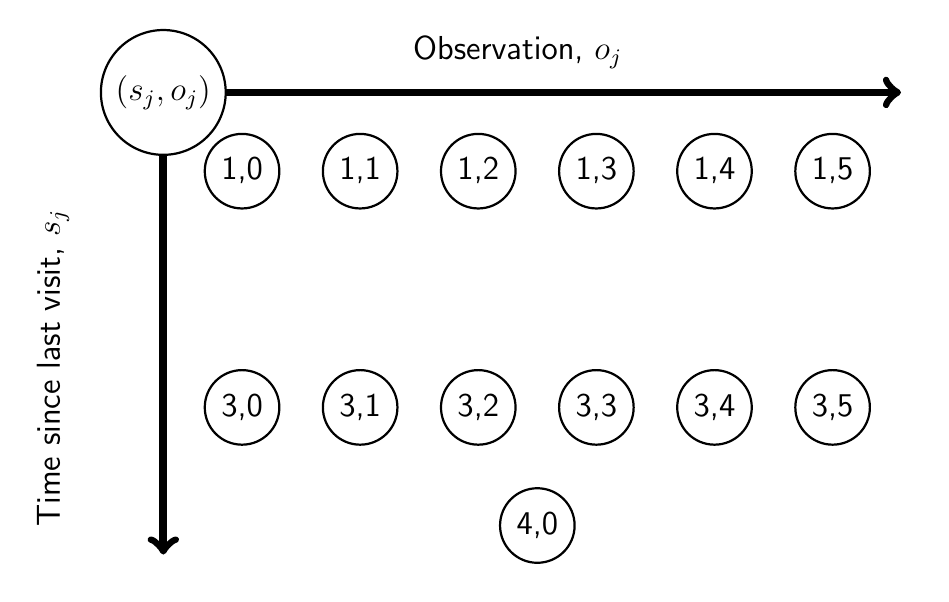
\begin{tikzpicture}[-,auto,node distance=1cm,
                    thick,main node/.style={circle,fill=white,draw,font=\sffamily\large,minimum size=0.5cm}]
 \foreach \x in {0,...,5}
    \foreach \y in {0,2} 
       {\pgfmathtruncatemacro{\label}{\x - 5 *  \y +21}
        \pgfmathtruncatemacro{\o}{\x}
        \pgfmathtruncatemacro{\s}{3-\y}
       \node [main node]  (\x\y) at (1.5*\x,1.5*\y) {\s,\o};}
       
\node[main node] (SpecialState) at (3.75,-1.5) {4,0};       

\node (XaxisLeft) [shift={(-0.5,1)}] at (02) {};
\node (XaxisRight) [shift={(1,1)}] at (52) {};

\node (YaxisBottom) [shift={(-1,-0.5)}] at (0,-1.5) {};
\node (YaxisTop) [shift={(-1,1)}] at (02) {};

\draw[->,line width=1mm] (XaxisLeft)--(XaxisRight);
\draw[->,line width=1mm] (YaxisTop)--(YaxisBottom);

\node[font=\sffamily\large] (OLabel) [shift={(0.5,1.5)}] at (22) {Observation, $o_{j}$};
\node[font=\sffamily\large] (SLabel) [shift={(-2.4,0.5)}] at (00) {\rotatebox{90}{Time since last visit, $s_{j}$}};

\node[main node] (Example) [shift={(-1,1)}] at (02) {$(s_{j},o_{j})$};

\end{tikzpicture}
\end{center}
\caption{Bernoulli with $b_{j}=5$, $x_{1,j}=3.1$ and $x_{2,j}=1.1$}
\end{myfigure}

We will be assuming that $\floor{x_{1}} \neq \floor{x_{2}}$ as otherwise it follows that only one $s_{j}$ survives and we fall into the deterministic category (bar some changes to the values) see Apendix \ref{Bernoulli Attack time with equal floors}.

Suppose we are in the state $(\floor{x_{1}}+1,o)$ for some $o=1,2,...,b$ then our decision is either to
\begin{itemize}
\item Visit now
\item Wait till we are in state $(\floor{x_{2}}+1,o)$ and then visit
\item Wait till we are in state $(\floor{x_{2}}+2,o)$ and then visit
\item Wait till we are in state $(\floor{x_{2}}+2,o)$ and wait
\end{itemize}

Now we write down the long-run average costs of following such a strategy
\begin{itemize}
\item Visit now:
\begin{equation}
\frac{c \lambda \int_{0}^{\floor{x_{1}}} P(X \leq t)dt +\omega}{\floor{x_{1}}+1}
=\frac{\omega}{\floor{x_{1}}+1}
\end{equation}
\item Wait till state $(\floor{x_{2}}+1,o)$ and then visit:
\begin{align}
&\frac{c \lambda \int_{0}^{\floor{x_{2}}} P(X \leq t)dt + coP(X \leq \floor{x_{2})})+\omega}{\floor{x_{2}}+1} \nonumber \\&=\frac{c \lambda (\floor{x_{2}}-x_{1})p +cop + \omega}{\floor{x_{2}}+1}
\end{align}


\item Wait till state $(\floor{x_{2}}+2,0)$ and then visit:
\begin{align}
&\frac{c \lambda \int_{0}^{\floor{x_{2}}+1} P(X \leq t)dt +coP(X \leq \floor{x_{2}}+1)+\omega}{\floor{x_{2}+2}} \nonumber \\ &=\frac{c \lambda ((x_{2}-x_{1})p + (\floor{x_{2}}+1-x_{2}))+co+\omega}{\floor{x_{2}}+2}
\end{align}

\item In state $(\floor{x_{2}}+2,0)$ waiting $k \geq 1$ then visiting:
\begin{align}
&\frac{c \lambda \int_{0}^{\floor{x_{2}}+1+k} P(X \leq t)dt +coP(X \leq \floor{x_{2}}+1+k)+\omega}{\floor{x_{2}+2+k}} \nonumber \\ &=\frac{c \lambda ((x_{2}-x_{1})p + (\floor{x_{2}}+1+k-x_{2}))+co+\omega}{\floor{x_{2}}+2+k}
\end{align}

\end{itemize}


Very similar to before we will look at when certain costs are better. Starting with Visit now beating all others if $ \omega < \frac{cp(\floor{x_{1}}+1)(\lambda (\floor{x_{2}}-x_{1})+o)}{\floor{x_{2}}-\floor{x_{1}}}$ and $\omega < \frac{c(\floor{x_{1}}+1)(\lambda (x_{2}-x_{1})p + (\floor{x_{2}}-x_{2}+1)+o)}{\floor{x_{2}}-\floor{x_{1}}+1}$ and $\omega < \frac{c(\floor{x_{1}}+1)(\lambda (x_{2}-x_{1})p + (\floor{x_{2}}-x_{2}+1+k)+o)}{\floor{x_{2}}-\floor{x_{1}}+1+k}$ for all $k \geq 1$. The first inequality guarantees the other two so we get

Visit now if:
\begin{equation}
\omega < \frac{cp(\floor{x_{1}}+1)(\lambda (\floor{x_{2}}-x_{1})+o)}{\floor{x_{2}}-\floor{x_{1}}}
\end{equation}

We can similarly find the visit in state $(\floor{x_{2}}+1,o)$ by requiring that $ \omega > \frac{cp(\floor{x_{1}}+1)(\lambda (\floor{x_{2}}-x_{1})+o)}{\floor{x_{2}}-\floor{x_{1}}}$ and $\omega < c (\lambda ( p( (x_{2}-x_{1})(\floor{x_{2}}+1)-(\floor{x_{2}}-x_{1})(\floor{x_{2}}+2)) + (\floor{x_{2}}-x_{2}+1)(\floor{x_{2}}+1)+o((1-p)(\floor{x_{2}}+1)-p))$ and $\omega < \frac{c}{k+1} (\lambda ( p( (x_{2}-x_{1})(\floor{x_{2}}+1)-(\floor{x_{2}}-x_{1})(\floor{x_{2}}+2+k)) + (\floor{x_{2}}-x_{2}+k+1)(\floor{x_{2}}+1)+o((1-p)(\floor{x_{2}}+1)-p(k+1)))$. Note the second inequality implies the third one, so

Visit in state $(\floor{x_{2}}+1,o)$ if:
\begin{align}
&\frac{cp(\floor{x_{1}}+1)(\lambda (\floor{x_{2}}-x_{1})+o)}{\floor{x_{2}}-\floor{x_{1}}} < \omega < \nonumber \\ &c (\lambda ( p( (x_{2}-x_{1})(\floor{x_{2}}+1)-(\floor{x_{2}}-x_{1})(\floor{x_{2}}+2)) + (\floor{x_{2}}-x_{2}+1)(\floor{x_{2}}+1)+o((1-p)(\floor{x_{2}}+1)-p)) \nonumber \\
&=c (\lambda (1-p)((\floor{x_{2}}-x_{2})(\floor{x_{2}}+1) + \floor{x_{2}}) + 1 +px_{1} +o((1-p)(\floor{x_{2}}+1)-p))
\end{align}

Again we could possible not have this region if the left hand side overlaps the right (but for now we will ignore it).

Again we can similarly find the visit in state $(\floor{x_{2}}+2,0)$ by requiring that
$ \omega > \frac{cp(\floor{x_{1}}+1)(\lambda (\floor{x_{2}}-x_{1})+o)}{\floor{x_{2}}-\floor{x_{1}}}$ and $\omega > c (\lambda ( p( (x_{2}-x_{1})(\floor{x_{2}}+1)-(\floor{x_{2}}-x_{1})(\floor{x_{2}}+2)) + (\floor{x_{2}}-x_{2}+1)(\floor{x_{2}}+1)+o((1-p)(\floor{x_{2}}+1)-p))$ and $\omega < c (\lambda (1+E[X])-o)$. Now the second inequality implies the first one (???? double check this ????), so

Visit in state $(\floor{x_{2}}+2,0)$ immediately if:
\begin{align}
&c (\lambda (1-p)((\floor{x_{2}}-x_{2})(\floor{x_{2}}+1) + \floor{x_{2}}) + 1 +px_{1} +o((1-p)(\floor{x_{2}}+1)-p)) \nonumber \\
&< \omega < c(\lambda (1+E[X])-o)
\end{align}

Again there is a possibility of overlap (but for now we will ignore it)

Finally we will never visit if:
\begin{equation}
\omega > c(\lambda (1+E[X])-o)
\end{equation}


\begin{example}
Suppose $x_{1}=0.1$,$x_{2}=2.1$ with $p=0.2$ and $b=5$, then our state space is reduced to $\Omega= \{ (1,o) \, | o=0,1,...,5 \} \cup \{ (1,o) \, | o=0,1,...,5 \} \cup \{ (4,0) \}$ and we make the decision at state $(1,o)$. We start by calculating the various critical regions, for which we will use $\lambda=20$ and $o=1$.

First critical value(Equation 12): $\frac{c(0+1)(20 \times (2-0.1)+1)}{2-0}=\frac{39c}{2}=19.5c$

Second critical value(Equation 13): $c(20 \times (1-0.2)((2-2.1)(2+1)+1)+1+0.2 \times 0.1 + 1 \times ((1-0.2)(2+1)-0.2))=14.42c$

Third critical value(Equation 14): $c(20 \times (1+ 0.2 \times 0.1+0.8 \times 2.1)-1)=53c$.

So in this case the decision will be based on the cost, $\omega$:
\begin{itemize}
\item Visit immediately if $\omega \leq 19.5c$
\item Wait till $(4,0)$ (three time periods) and visit immediately if $19.5c <\omega < 53c$
\item Never visit if $\omega \geq 53c$
\end{itemize}
\end{example}

\subsection{Correction to approach for bernoulli}
We will first have a concrete argument as to why we can renew all states, $(s,v)$ with $s < \floor{x_{1}}+1$. From this position consider the policy which waits $k$ time periods and then renews and follows the optimally policy, $\sigma$, with $k=0,...,\floor{x_{1}}+1-s$.

Using such a policy will get us that
\begin{equation}
V_{n}^{\pi_{k}}(s,v)=\omega+E[V_{n-k-1}^{\sigma}(\theta)]
\end{equation}
Where $\theta$ is the state upon renewal (i.e the state $(1,V) \sim (1,TPo(\lambda)$)

Now we will pick policy $\pi_{k+1}$ over $\pi_{k}$ (or be indifferent) if

\begin{align*}
&\lim\limits_{n \rightarrow \infty} V_{n}^{\pi_{k}} (s,v) - V_{n}^{\pi_{k+1}}(s,v) \geq 0 \\
& \iff \lim\limits_{n \rightarrow \infty} E[V_{n-k-1}^{\sigma}(\theta) - V_{n-k-2}^{\sigma} (\theta)] \geq 0 \\
& \iff g \geq 0
\end{align*}

Where $g$ is the average long-run costs of the system, coming from $V_{n}=ng+\phi(s,v)$ for large n, where $\phi(s,v)$ is some initial bias for not starting in the equilibrium but from the initial state $(s,v)$.

Now as the Dynamic Programming only have positive costs, it is impossible for $g < 0$. So we have $g \geq 0 $, so it is better to pick policy $\pi_{k+1}$ over $\pi_{k}$ , as the argument holds for all $k=0,...,\floor{x_{1}}+1-s$ (and all $v$) it is best to wait till $(\floor{x_{1}}+1,v)$ before making a decision, i.e if we are too renew we might as well renew at $(\floor{x_{1}}+1,v)$ (though we might not renew here).

This formally shows the removal of the initial section of states (i.e those at the top).

Now we will skip to the state $(\floor{x_{2}}+2,0)$ and again suggest a policy, $\pi_{k}$ which waits $k$ time periods before renewing and then follows some optimal policy, $\sigma$.

Using such as policy will get us
\begin{align*}
V_{n}^{\pi_{k}}(s,v)&=\omega + c \lambda p  k + c \lambda (1-p) k + E[V_{n-k-1}^{\sigma}(\theta)] \\
&=\omega + c \lambda k + E[V_{n-k-1}^{\sigma}(\theta)] 
\end{align*}

so we will pick policy $\pi_{k+1}$ over $\pi_{k}$ (or be indifferent) if

\begin{align*}
&\lim\limits_{n \rightarrow \infty} V_{n}^{\pi_{k}}(s,v) - V_{n}^{\pi_{k+1}}(s,v) \geq 0 \\
& \iff \lim\limits_{n \rightarrow \infty} -c \lambda + E[V_{n-k-1}^{\sigma}(\theta) - V_{n-k-2}^{\sigma} (\theta)] \\
& \iff -c \lambda + g \geq 0 \\
& \iff f \geq c \lambda
\end{align*}

So hence if $g \geq c \lambda$ we will wait forever, as this has no dependence on $k$.

We will now argue that $g_{\text{max}}= c \lambda$, that is the worst long-run average cost is $c \lambda$. This can be be seen by the strategy, $\pi_{\text{neg}}$, a strategy which never renews no matter what state we are in. I.e the patroller neglects the node. We will have that, for large $n$

\begin{align*}
V_{n}^{\pi_{\text{neg}}}(s,v)= n c \lambda + \phi(s,v)
\end{align*}
We can observe this by looking at the actual decay of the process under a policy that never renews

\begin{align*}
V_{n}^{\pi_{\text{neg}}}(s,v)&= \begin{cases}
n c \lambda \text{ If } s \geq \floor{x_{2}}+2 \\
V_{n-(\floor{x_{2}}+2-s)} + \phi(s,v) \text{ If }  s \leq \floor{x_{2}}+1
\end{cases} \\
&= \begin{cases}
n c \lambda \text{ If } s \geq \floor{x_{2}}+2 \\
(n-(\floor{x_{2}}+2-s)) c \lambda + \phi(s,v) \text{ If }  s \leq \floor{x_{2}}+1
\end{cases} \\
\end{align*}

where

\begin{align*}
\phi(s,v)=&\begin{cases}
\underbrace{v c }_{\text{Observed finishing}} + \underbrace{c \lambda p (\floor{x_{2}}-x_{1}+1)}_{ x_{1} \text{ type attackers finishing}} + \underbrace{c \lambda (1-p) (\floor{x_{1}}-x_{1}+1)}_{ x_{2} \text{ type attackers finishing}} \text{ If } s \leq \floor{x_{1}}+1  \\
\underbrace{v c (1-p)}_{\text{Observed } x_{2} \text{ types finishing}} + \underbrace{c \lambda p (\floor{x_{2}}-x_{1}+1-s)}_{ x_{1} \text{ type attackers finishing}} + \underbrace{c \lambda (1-p) (\floor{x_{1}}-x_{1}+1)}_{ x_{2} \text{ type attackers finishing}} \text{ If } \floor{x_{1}}+2 \leq s \leq \floor{x_{2}}+1 \\
0 \text{ If } s \geq \floor{x_{2}}+2 
\end{cases} \\
&=\begin{cases}
v c + c \lambda (\floor{x_{2}}-x_{2}+1) + c \lambda p (x_{2}-x_{1}) \text{ If } s \leq \floor{x_{1}}+1  \\
v c p + c \lambda (\floor{x_{2}}-x_{2}+1) + c \lambda p (x_{2}-x_{1}-s) \text{ If } \floor{x_{1}}+2 \leq s \leq \floor{x_{2}}+1 \\
0 \text{ If } s \geq \floor{x_{2}}+2 
\end{cases}
\end{align*}

is the `transfer'/bias from the initial state to $(\floor{x_{2}}+2,0)$.

Hence for any service cost, $\omega$ we can achieve a $g= c \lambda$. So we will always be in the case of $g \leq c \lambda$ and hence will renew if we hit the state $(\floor{x_{2}}+2,0)$.

Now in this cases of $g \leq c \lambda$ (where we will not just follow neglection) we need to make a decision about what to do at states $(s,v)$ for $\floor{x_{1}}+1 \leq s \leq \floor{x_{2}}+1$, $0 \leq v \leq b$.

The real question again is how long we wait, before renewal. Let us suppose we are in one of these states $(s,v)$ then we notice that we will have slightly different costs depending which region we are in and how long we wait. We again use $\pi_{k}$ be the policy to wait $k$ ($k=0,1,...,\floor{x_{2}}-\floor{x_{2}}+1$) time units before renewing and then following some optimal policy, $\sigma$.

If we are in $(\floor{x_{1}}+1,v)$ then we will get

\begin{align*}
V_{n}^{\pi_{k}}(\floor{x_{1}}+1,v)&= \begin{cases}
\omega + E[V_{n-k-1}^{\sigma}(\theta)] \text{ If } k=0 \\
\omega + v c p + c \lambda p (\floor{x_{1}}-x_{1}+1+(k-1)) + E[V_{n-k-1}^{\sigma}(\theta)] \text{ If } 1 \leq k \leq \floor{x_{2}}-\floor{x_{1}} \\
\omega+ vc + c \lambda p (\floor{x_{1}}-x_{1}+1+\floor{x_{2}}-\floor{x_{1}}) + c \lambda (1-p) (\floor{x_{2}}-x_{2}+1) + E[V_{n-k-1}^{\sigma}(\theta)] \text{ If } k= \floor{x_{2}}-\floor{x_{1}}+1
\end{cases} \\
&=\begin{cases}
\omega + E[V_{n-1}^{\sigma}(\theta)] \text{ If } k=0 \\
\omega + v c p + c \lambda p (\floor{x_{1}}-x_{1}+1+(k-1)) E[V_{n-k-1}^{\sigma}(\theta)] \text{ If } 1 \leq k \leq \floor{x_{2}}-\floor{x_{1}} \\
\omega+ vc + c \lambda p (x_{2}-x_{1}) + c \lambda (\floor{x_{2}}-x_{2}+1) \text{ If } k= \floor{x_{2}}-\floor{x_{1}}+1
\end{cases}
\end{align*}

If we are in $(s,v)$ for $1 \leq s \leq \floor{x_{2}}$

\begin{align*}
V_{n}^{\pi_{k}}(\floor{x_{1}}+1,v)&= \begin{cases}
\omega + c \lambda p k + E[V_{n-k-1}^{\sigma}(\theta)] \text{ If } 0 \leq k \leq \floor{x_{2}}-\floor{x_{1}}-s \\
\omega+ vc(1-p) + c \lambda p (\floor{x_{2}}-\floor{x_{1}}-s+1) + c \lambda (1-p) (\floor{x_{2}}-x_{2}+1) + E[V_{n-k-1}^{\sigma}(\theta)] \text{ If } k= \floor{x_{2}}-\floor{x_{1}}+1-s+1
\end{cases} \\
&=\begin{cases}
\omega + c \lambda p k E[V_{n-k-1}^{\sigma}(\theta)] \text{ If } 0 \leq k \leq \floor{x_{2}}-\floor{x_{1}}-s \\
\omega+ vc(1-p) + c \lambda p (x_{2}-\floor{x_{1}}-s) + c \lambda (\floor{x_{2}}-x_{2}+1) \text{ If } k= \floor{x_{2}}-\floor{x_{1}}-s+1
\end{cases}
\end{align*}

If we are in $(\floor{x_{2}}+1,v)$ 

\begin{align*}
V_{n}^{\pi_{k}}(\floor{x_{2}}+1,v)&= \begin{cases}
\omega + E[V_{n-k-1}^{\sigma}(\theta)] \text{ If } k=0 \\
\omega+ vc(1-p) + c \lambda p + c \lambda (1-p) (\floor{x_{2}}-x_{2}+1) + E[V_{n-k-1}^{\sigma}(\theta)] \text{ If } k= 1
\end{cases} \\
&=\begin{cases}
\omega + E[V_{n-k-1}^{\sigma}(\theta)] \text{ If } k=0 \\
\omega+ vc(1-p) + c \lambda p (x_{2}-\floor{x_{2}}) + c \lambda (\floor{x_{2}}-x_{2}+1) + E[V_{n-k-1}^{\sigma}(\theta)] \text{ If } k= 1
\end{cases}
\end{align*}

We now seek to compare policies for states, we we shall start with the state, $(\floor{x_{2}}+1,v)$ then we will pick policy $\pi_{0}$ over $\pi_{1}$ if

\begin{align*}
&\lim\limits_{n \rightarrow \infty} V_{n}^{\pi_{1}}(\floor{x_{2}}+1,v) - v_{n}^{\pi_{0}} (\floor{x_{2}}+1,v) \geq 0 \\
& \iff \lim\limits_{n \rightarrow \infty} \omega+ vc(1-p) + c \lambda p (x_{2}-\floor{x_{2}}) + c \lambda (\floor{x_{2}}-x_{2}+1) + E[V_{n-2}^{\sigma}(\theta)]-(\omega + E[V_{n-1}^{\sigma}(\theta)]) \\
& \iff \lim\limits_{n \rightarrow \infty} E[V_{n-2}^{\sigma}(\theta)-V_{n-1}^{\sigma}(\theta)] + vc(1-p)+ c \lambda p(x_{2}-\floor{x_{2}}) + c \lambda (\floor{x_{2}}-x_{2}+1) \\
& \iff g \leq vc(1-p)+ c \lambda p(x_{2}-\floor{x_{2}})) + c \lambda (\floor{x_{2}}-x_{2}+1)
\end{align*}

So we will renew immediately in $(\floor{x_{2}}+2,0)$ from here if $ g \leq vc(1-p)+ c \lambda p(x_{2}-\floor{x_{2}})) + c \lambda (\floor{x_{2}}-x_{2}+1) $. We will use $R_{2}=x_{2}-\floor{x_{2}}$ ($0 \leq R_{2} < 1$).

So to have the possibility to wait and renew we will need that $vc(1-p) + c \lambda p R_{2} + c \lambda (1-R_{2}) \leq c \lambda \iff c(1-p)(v-R_{2} \lambda) \leq 0 \iff v- R_{2} \lambda \leq 0 \iff v \leq R_{2} \lambda$.

\begin{note}
We note that this sort of result is analogous to the deterministic case.
\end{note}

now we note that we can again create a $v_{\text{crit}}(\floor{x_{2}}+1)$, from which we will renew immediately for all  $v \geq v_{\text{crit}}(\floor{x_{2}}+1)$ and for $v < v_{\text{crit}}(\floor{x_{2}}+1)$ we wait.

We rearrange $g \geq vc(1-p)+ c \lambda p(x_{2}-\floor{x_{2}})) + c \lambda (\floor{x_{2}}-x_{2}+1)$ to get $v_{\text{crit}}(\floor{x_{2}}+1)=\ceil{\frac{g}{c(1-p)}- \frac{\lambda}{(1-p)} -\lambda R_{2}}$.

We again know that, $g_{\text{max}}= c \lambda$ so we get the maximum $v_{\text{crit}}=\ceil{\frac{c \lambda}{c (1-p)} - \frac{\lambda}{(1-p)}- \lambda R_{2}}=\ceil{\lambda R_{2}}$

So when $R_{2}=0$ then we immediately renew and will never wait in the state $(\floor{x_{2}}+1,v)$ for any $v$.


\section{Ideas for future}
\begin{itemize}
\item Extend $X$ to be a binomial distribution
\item Extend $X$ to be any discrete distribution
\item Extend $X$ to be a normal distribution by approximation to binomial
\item Test Deterministic case against strategic attacker (non-random) on extended star graph
\end{itemize}
%End of main part of document
\bibliography{mybib}

\appendix
\pagenumbering{roman}
\appendixpage
\addappheadtotoc
\section{Observations are always zero}
\label{Observations are always zero}

On a single node we are limited to the state space of $\Omega=\{ (1,0),...,(\floor{B}+2,0) \}$, then on this state space we can implement a policy which returns every $k$ time units, this will gives an average long run cost of

\begin{equation}
f(k)=\frac{c \lambda \int_{0}^{k-1} P(X \leq t) dt +\omega}{k}
\end{equation}

So to find out when the patroller would be indifferent from choosing to return every $k$ or every $k+1$, solve $f(k+1)-f(k)=0$ giving

$$\frac{1}{k(k+1)}(c \lambda (k \int_{k-1}^{k} P(X \leq t) dt - \int_{0}^{k-1} P(X \leq t) dt ) -\omega)=0 $$

Prompting an index of

$$W(k)=c \lambda (k \int_{k-1}^{k} P(X \leq t) dt - \int_{0}^{k-1} P(X \leq t) dt )$$

We note that $W(0)=0$ and for $k \geq B+1$ $W(k)=c \lambda (k - int_{0}^{k+1} P(X \leq t)dt=c \lambda (1+\int_{0}^{k-1} P(X > t)dt)=c \lambda (1+ E[X])$. We will now show that:
\begin{itemize}
\item $W(k)$ is non-decreasing
\item The optimal policy when $\omega \in [W(k-1),W(k)]$ is to visit every k time units
\item If $w \geq c \lambda (1+E[X])$ then it is optimal to never visit
\end{itemize}

\begin{proof}
First
\begin{align*}
W(k+1)-W(k)&= c \lambda ((k+1) \int_{k}^{k+1} P(X \leq t)dt - \int_{0}^{k} P(X \leq t)dt \\ & \quad \quad \quad -(k \int_{k-1}^{k} P(X \leq t)dt - \int_{0}^{k-1} P(X \leq t)dt)) \\ &=c \lambda ((k+1) \int_{k}^{k+1} P(X \leq t)dt -k \int_{k-1}^{k} P(X \leq t)dt - \int_{k}^{k-1} P(X \leq t)dt)\\ &=c \lambda (k+1) (\int_{k}^{k+1} P(X \leq t)dt - \int_{k-1}^{k} P(X \leq t)dt) \geq 0
\end{align*}

As $P(X \leq t)$ is non-decreasing.

Second if $\omega \in [W(k-1),W(k)]$ then we will show that $f(m)$ is non-increasing for $m \leq k$ and non-decreasing for $m \geq k$.

For $m \leq k$
\begin{align*}
f(m)-f(m-1)&=\frac{1}{m(m-1)}(c \lambda (m-1) \int_{0}^{m-1} P(X \leq t) dt - c \lambda m \int_{0}^{m-2} P(X \leq t) dt - \omega) \\
&=\frac{1}{m(m-1)}(W(m-1)-\omega) \leq \frac{1}{m(m-1)} (W(m-1)-W(k-1)) \leq 0
\end{align*}

Similarly for $m \geq k$
\begin{align*}
f(m+1)-f(m)&= \frac{1}{m(m+1)} (W(m)-\omega) \geq \frac{1}{m(m+1)} (W(m)-W(k)) \geq 0
\end{align*}
Hence choosing to visit every $k$ time units is optimal.

Third and finally our upper limit of $c \lambda (1+E[X])$ (Which is $W(k)$ for $k \geq B+1$) means we are indifferent from picking $k$ and $k+1$ for $k \geq B+1$ so we will never visit. I.e
$f(k+1) \leq f(k) \iff w \geq W(k)$ so not optimal if $f(k+1) \geq f(k) \, \forall k \iff w \geq \sup\limits_{k=1,2,...} W(k)=\lim\limits_{k \rightarrow \infty} W(k)=c \lambda (1+E[X])$
\end{proof}

\section{Bernoulli Attack time with equal floors}
\label{Bernoulli Attack time with equal floors}

If we have $\floor{x_{1}}=\floor{x_{2}}$ then $\Omega= \{(\floor{x_{1}}+1,o) \, | \, o=0,1,...,b \} \cup \{(\floor{x_{1}}+2,o) \}$

Suppose we are in the state $(\floor{x_{1}}+1,o)$ for some $o=1,2,...,b$ then our decision process is the same as the deterministic case
\begin{itemize}
\item Visit now
\item Wait till we are in state $(\floor{x_{1}}+2,0)$ and wait for $k$ time units before visiting, $k \geq 0$
\end{itemize}

We again write down long-run average costs of following such a strategy
\begin{itemize}
\item Visit now:
\begin{equation}
\frac{c \lambda \int_{0}^{\floor{x_{1}}} P(X \leq t) dt + \omega}{\floor{x_{1}}+1}=\frac{\omega}{\floor{x_{1}}+1}
\end{equation}
\item Wait till state $(\floor{x_{1}}+2,0)$ then wait $k \geq 0$ time units before visiting:
\begin{align}
&\frac{c \lambda \int_{0}^{\floor{x_{1}}+1+k} P(X \leq t) dt + coP(X \leq \floor{x_{1}}+1+k) +\omega }{\floor{x_{1}}+2+k} \nonumber \\ &=\frac{c \lambda (p(x_{2}-x_{1})+(\floor{x_{1}}+1+k-x_{2})) + co + \omega}{\floor{x_{1}}+2+k}
\end{align}
\end{itemize}

Now to visit now we will only do so if $\omega < c (\floor{x_{1}}+1) (\lambda (p\frac{x_{2}-x_{1}}{k+1}+ (\frac{\floor{x_{1}}-x_{2}}{k+1} +1))+\frac{o}{k+1})$ for all $k \geq 0$, We need to know if $\lambda (\floor{x_{1}}-px_{1}+px_{2}-x_{2})+o \begin{cases}
 >0 \\
 <0
\end{cases}$. 
In the first case we get to visit if:
\begin{equation}
\omega < c(\floor{x_{1}}+1)(\lambda (\floor{x_{1}}-px_{1}+px_{2}-x_{2}+1)+ o)
\end{equation}
In the second case we get to visit if:
\begin{equation}
\omega < c \lambda (\floor{x_{1}}+1)
\end{equation}



If we do no visit initially then we will visit once transitioned and waited $k+1$ over $k$ if $\omega > c (\lambda (1+E[X])-o)$.

For in between values (dependent on which case) we will get that we will transition and visit immediately.
I.e if
First case
\begin{equation}
c(\floor{x_{1}}+1)(\lambda (\floor{x_{1}}-px_{1}+px_{2}-x_{2}+1)+ o) < \omega < c (\lambda (1+E[X])-o) 
\end{equation}
Second case
\begin{equation}
c \lambda (\floor{x_{1}}+1) < \omega < c (\lambda (1+E[X])-o)
\end{equation}

Again these regions may or may not exist dependent on their conditions.

\end{document}
